
\documentclass[11pt,parskip=full]{report}
\usepackage[Bjornstrup]{fncychap}
\usepackage{pkgAndStyle}

\usepackage[utf8]{inputenc}
\usepackage[english]{babel}
\usepackage{amsmath}
\usepackage{amsfonts}
\usepackage{amssymb}
\usepackage{mathtools}
\usepackage{graphicx,wrapfig,lipsum}
% the wrapfig can easily put images at a side of the text

\usepackage{fancyhdr}
\usepackage{hyperref}
\usepackage{subcaption}
\usepackage{comment}
\usepackage{csquotes} %quotes
\usepackage{natbib}% for the bibliography
\usepackage[colorinlistoftodos]{todonotes}
\usepackage{xr}	
\usepackage{listings}
\usepackage{stackengine} % to write text below the images without number
\usepackage{color}
\usepackage{mathtools}
\DeclarePairedDelimiter\ceil{\lceil}{\rceil} %for the ceil operator
\DeclarePairedDelimiter\floor{\lfloor}{\rfloor}




\author{Nicola Covallero}
\title{Master Thesis}
\date{\today}
\begin{document}
\maketitle
\pagebreak
\tableofcontents
\pagebreak

\chapter{Abstract}


\chapter{Introduction}
\label{ch:introduction}

Robotic manipulation of objects is an increasing field of research which has struggled researches from many years ago. In several industries environments robots can be easily programmed considering some standard objects, i.e. the manipulation is always the same and known, and usually robot operations avoid to deal in cluttered scene, for instance through a conveyor belt the objects are singulated from the others ones. In order to move the robots outside industries and bring them to home of people they need to be equipped with a particular intelligence and skills that are still at a first stage.
In this thesis we are going to investigate a simple approach that tries to replicate the human reasoning step during the manipulation of objects of table clearing task. The main objective is trying also to manipulate the objects in a human style, that is paying attention that during the manipulation the collision between objects is avoid as much as possible. This is a behaviour that all we do, of course with fragile objects, but also with objects that have no problem regarding collisions.  

Next, in this chapter a brief introduction of the problem and the approach used is commented, and the experimental set up as well since it will be useful to understand some techniques and choice for the algorithm. 

\section{Problem Approach}
In this section the approach to resolve the planning problem is described. All the strategy is inspired to a human like solution. A human to resolve such a task would use three main actions: grasp an object with one hand or both, when it is not possible to grasp an object because other object imped the human to put the hands in the proper way to grasp a desired object he/she has to interact with the objects in order to achieve a configuration of the objects that can be suitable to grasp an object, and this is achieved through pushing or dragging actions. Dragging an object is a very complex action which will need the robot to lay the end effector on the top of an object and make enough pressure on the contact in order that the friction between the table and the object is minor than the friction between the object and the robot's end effector. This is a very hard action which would imply an implementation of a reliable controller, because the goal is not only to move the object but also not to ruin it.  

For these considerations the main actions the robot has to use in order to interact with the objects are:
\begin{itemize}
\item Grasping
\item Pushing
\end{itemize}
Grasping is the most important action since it lets to take an object from the pile of objects and drop it somewhere, for example in a bin, clearing in this way the table. There exist different works facing the same task by focusing only in grasping. The pushing becomes useful considering the problem that two adjacent objects could not be grasped if they are so close such that the robot's gripper, when attempting to grasp an object is going to collide with an adjacent object, making such an object ungraspable. From this consideration is necessary the pushing action, in order to separate adjacent objects which could mutually exclude themselves to be grasped. Moreover the robot's intelligence is enhanced by a planning system which will return a sequence of actions in order to achieve the goal to clear the table.  

\section{Set Up}
In order to make the understanding of the approach used the name the set up of the environment the robot will work in is presented. 
The robot used is a Barret WAM arm, which is a 7 degree of freedom (DoF) manipulator arm shown in Figure \ref{fig:wam_1}. 

\begin{figure}[htp]
\centering
\begin{subfigure}[b]{0.45\textwidth}
\centering
\includegraphics[height=5cm]{Img/set_up/wam.jpg}
\caption{Barrett WAM arm}\label{fig:wam_1}
\end{subfigure}
\begin{subfigure}[b]{0.45\textwidth}
\centering
\includegraphics[width=5cm]{Img/set_up/Kinect.jpg}
\caption{Microsoft Kinect sensor}\label{fig:wam_1}
\end{subfigure}
\caption{Robot and vision sensor.}
\end{figure}

This robot is characterized by a low inertia of the end effector thanks to the kind of its actuators. The WAM is noteworthy because it does not use any gears for manipulating the joints, but rather a cable drive, so there are no backlash problems and it is both fast and stiff. Cable drives permit low friction and ripple-free torque transmission from the actuator to the joints. 




To manipulate the objects the manipulation skills of the robot are enhanced by a gripper designed in the IRI institute driven by Dynamixel motors. Such a gripper is depicted in Figure \ref{fig:gripper_general} from several point of views. 

\begin{figure}[htp]
\centering
\begin{subfigure}[b]{0.3\textwidth}
\centering
\includegraphics[height=3cm]{Img/set_up/gripper1.png}
%\caption{}
\end{subfigure}
\begin{subfigure}[b]{0.3\textwidth}
\centering
\includegraphics[height=3cm]{Img/set_up/gripper2.png}
%\caption{}
\end{subfigure}
\begin{subfigure}[b]{0.3\textwidth}
\centering
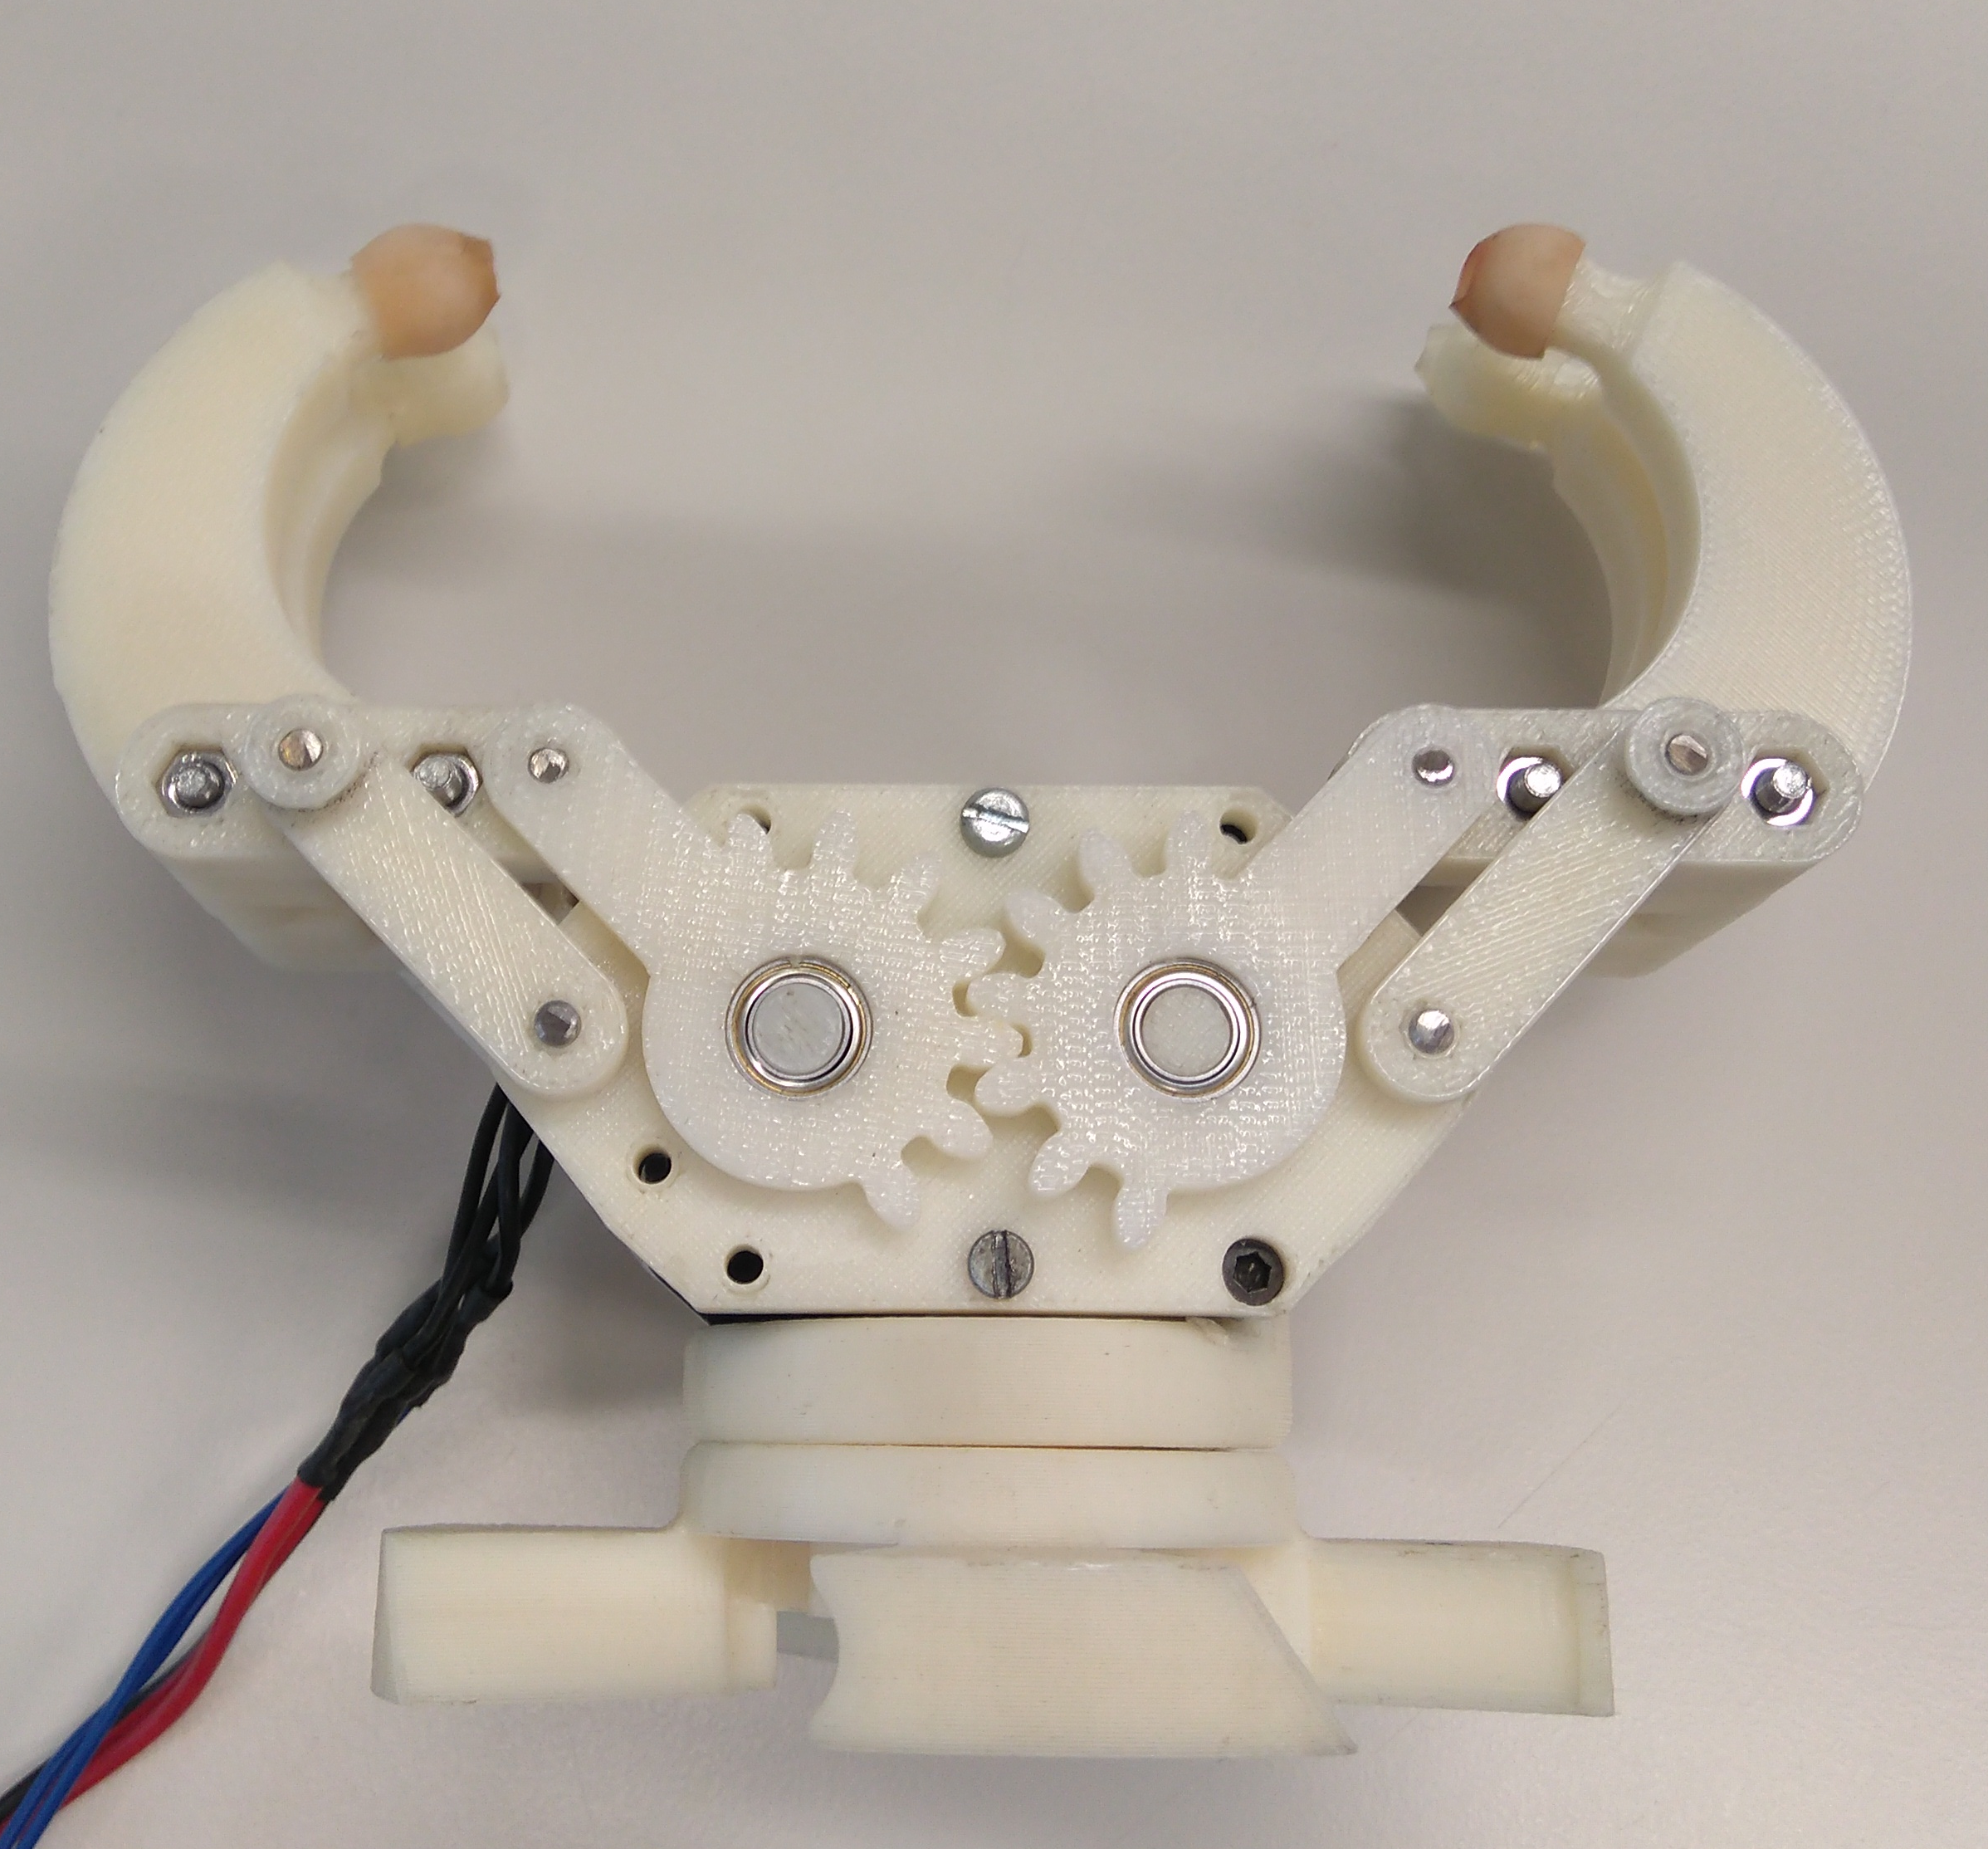
\includegraphics[width=3cm]{Img/set_up/gripper3.png}
%\caption{}
\end{subfigure}
\caption{Gripper used for the experiments}\label{fig:gripper_general}
\end{figure}

For the task planner, as the reader will see in chapters \ref{ch:task_planner} and \ref{ch:algorithm}, the model of the gripper will be an important resource 
in order to find a feasible sequence of action that can free the table.

The gripper will be modelled measuring some principal elements such as: finger's width and height, gripper's width, height and deep, and the distance between the fingers when the gripper is opened or closed. The modelling procedure is depicted in Figure \ref{fig:gripper_modelling}. The resulting model is a simple polygonal mesh which includes all the important geometric information of the gripper.

\begin{wrapfigure}{r}{6.5cm}
\caption{Gripper and WAM.}\label{fig:wam_gripper}
\includegraphics[width=5.0cm]{Img/set_up/wam_gripper.png}
\end{wrapfigure}

Such a simple model allows the collision algorithm commented in chapter \ref{ch:algorithm} to check for collision in just few millisecond. 
A more detailed and complex model would only lead as benefits a higher precision, precision that in this case is not needed, and it will slow down algorithm because the collision checking procedure would be more computationally expensive. 
The gripper will be mounted in the end effector of the robot as shown in Figure \ref{fig:wam_gripper}. 


\begin{figure}[htp]
\centering
\begin{subfigure}[t]{0.25\textwidth}
\centering
\stackunder[5pt]	{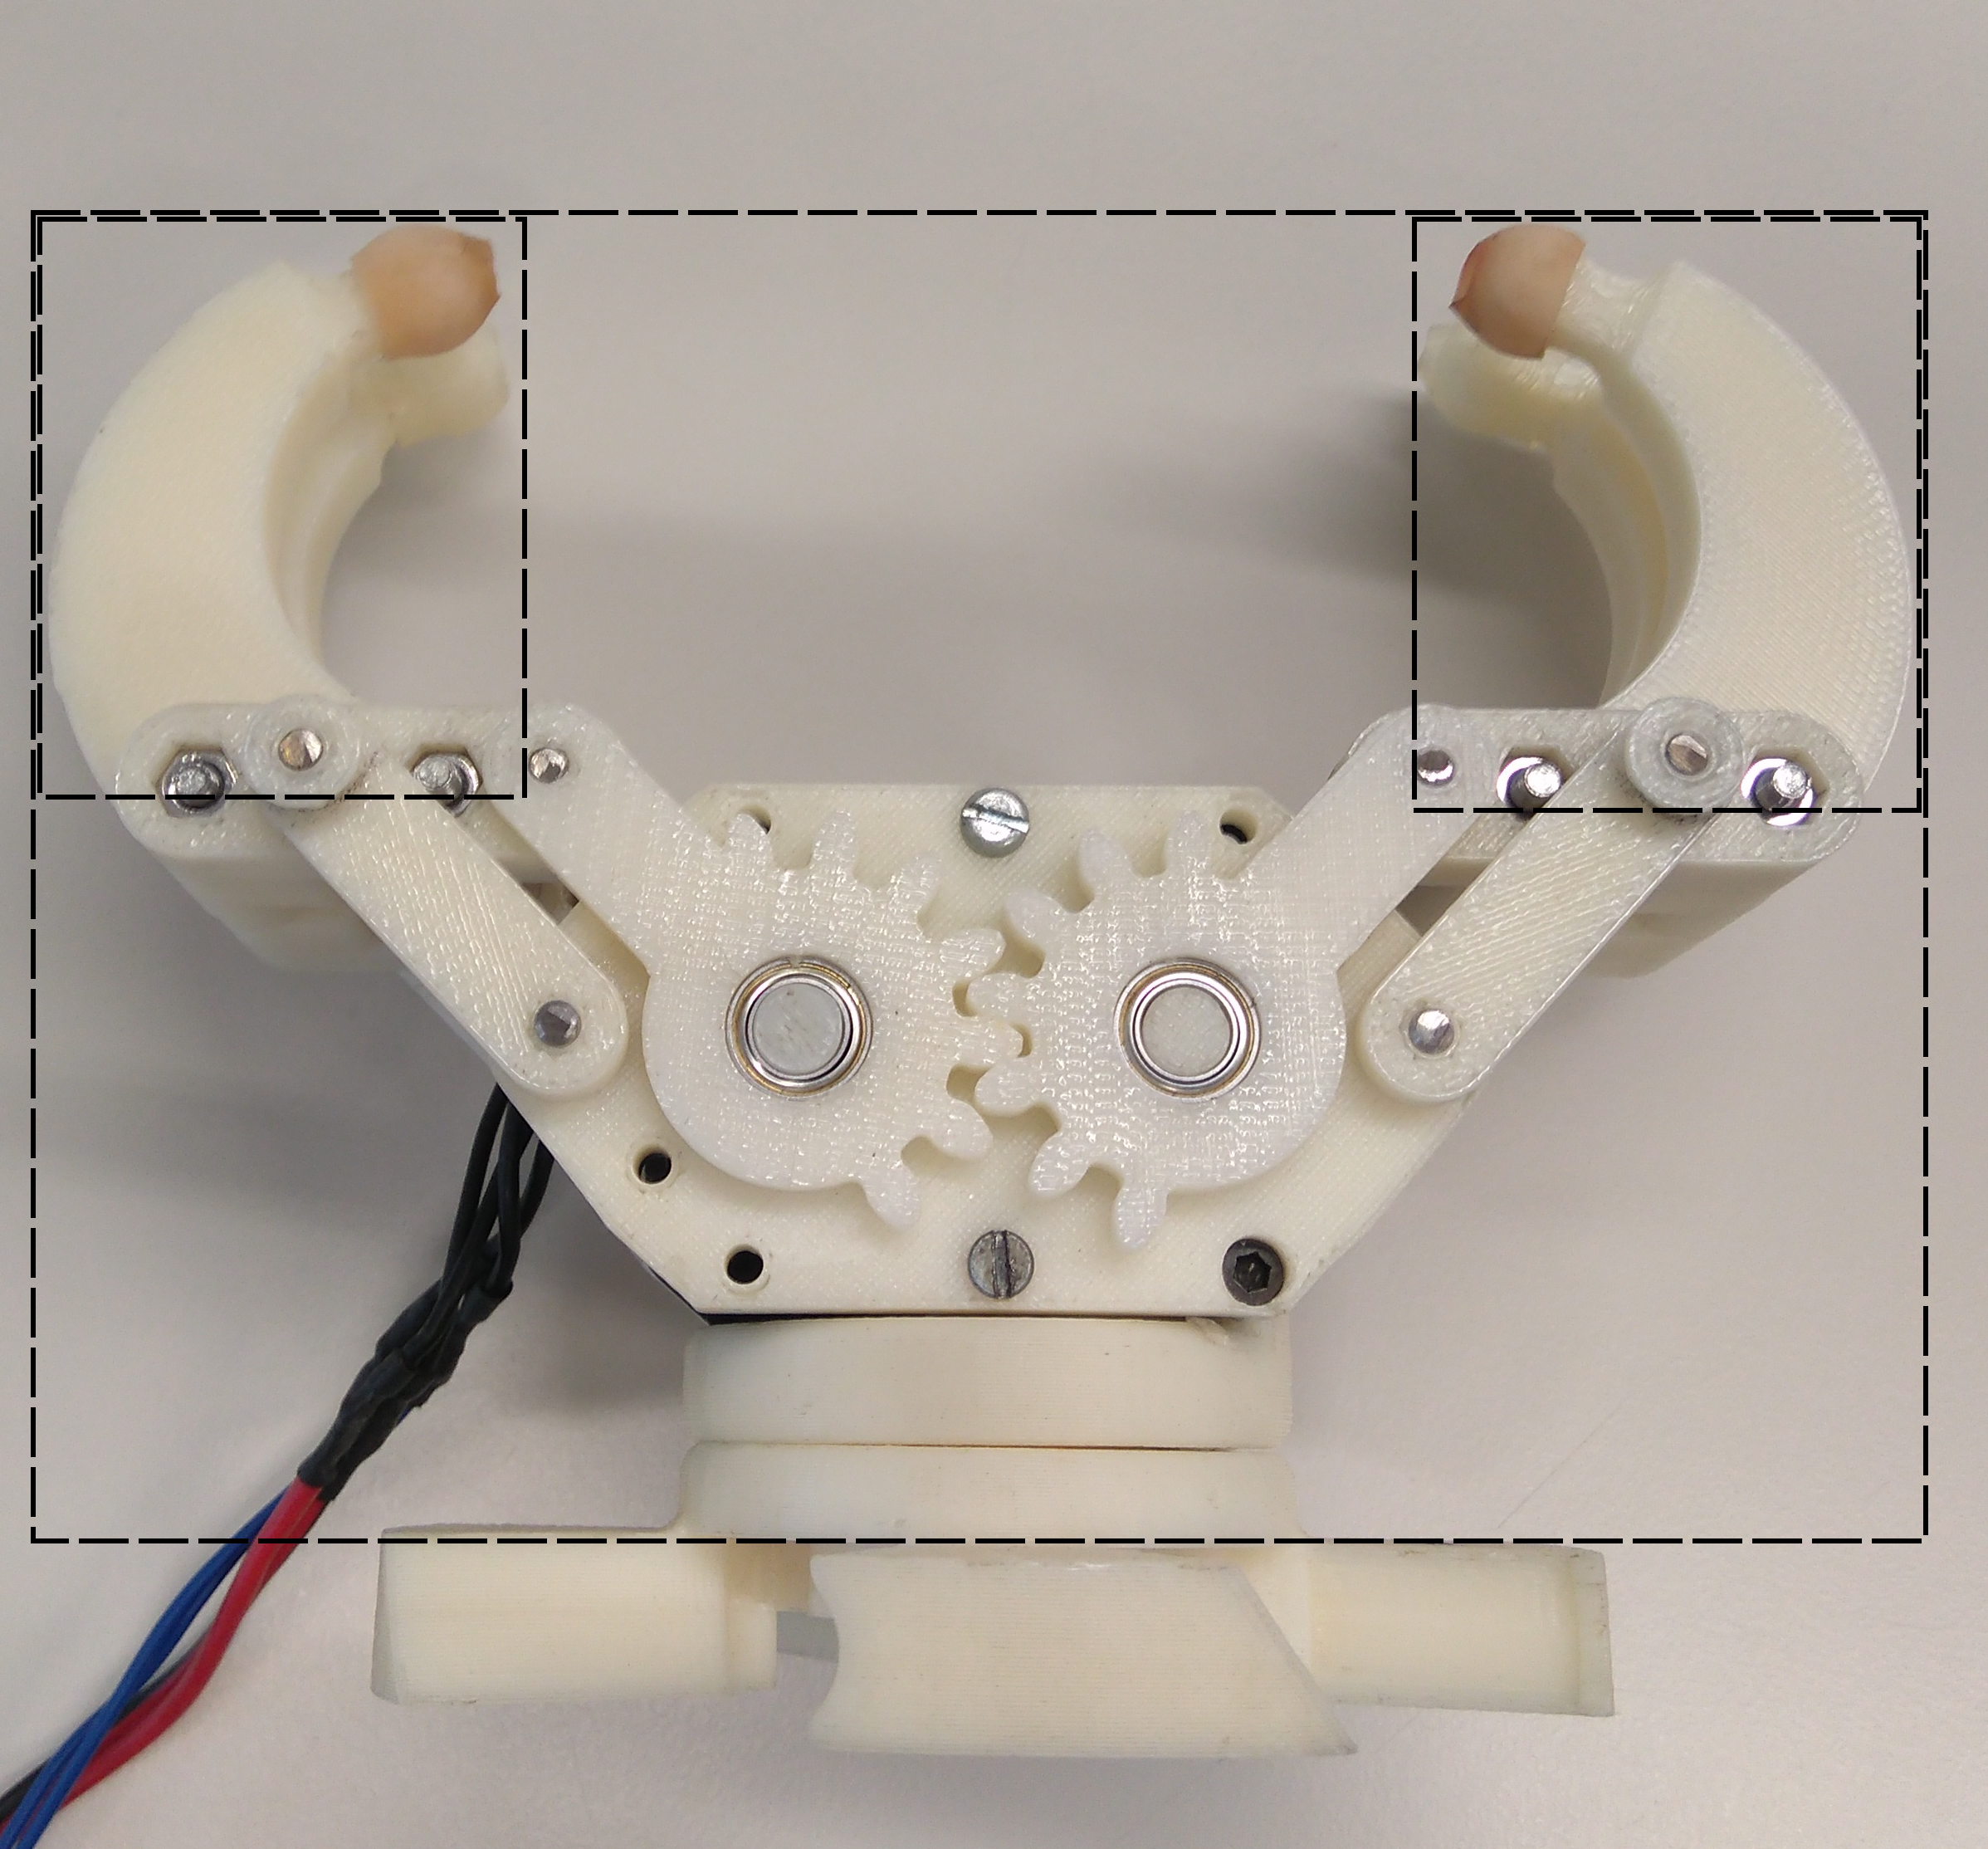
\includegraphics[height=3cm]{Img/set_up/gripper_modelling1.png}}{Elements measured}
\end{subfigure} 
\begin{subfigure}[t]{0.3\textwidth}
\centering
\stackunder[5pt]	{\includegraphics[height=3cm]{Img/set_up/gripper_open_model.png}}{Opened gripper mesh model}
\end{subfigure}
\hspace{1cm}
\begin{subfigure}[t]{0.3\textwidth}
\centering
\stackunder[5pt]	{\includegraphics[height=3cm]{Img/set_up/gripper_closed_model.png}}{Closed gripper mesh model}
%\caption{}
\end{subfigure}
\caption{Modelling of the gripper: the fingers width, fingers height, the height of the whole gripper, its width and its deep have been measured. The \textcolor{red}{red}, \textcolor{green}{green} and \textcolor{blue}{blue} axis are respectively the x, y and z axis.}\label{fig:gripper_modelling}
\end{figure}

The scenario the robot is going to work in is presented by a table, and the objects will lay on top of it. In Figure \ref{fig:setup_} the main elements of are highlighted. The WAM arm is in a fixed position with respect the table and the Kinect camera is located on top of the table pointing down. The Kinect is calibrated and the fixed transformation between the Kinect's frames and the base frame of the robot is known, so all the points measured by the Kinect can be expressed in coordinates with respect the robot's frame. An example of a cluttered scene the robot is going to deal with is depcited in Figure \ref{fig:example_scene}, and the same scene seen by the Kinect is shown in Figure \ref{fig:kinect_view}. With respect the kinect's view the robot is located at the top of the image, outside the point of view of the Kinect in order to avoid to detect the arm as an object. If the robot arm would be present in a depth image we should apply some algorithms to identify the robot arm, which could also produce important occlusions, that is hide some objects from the Kinect's view. In order to avoid all this, the depth image considered is the last one provided by the Kinect when the robot is no more in the Kinect's view (these poses are known a priori). 

\begin{figure}[htp]
\centering
\begin{subfigure}[b]{0.4\textwidth}
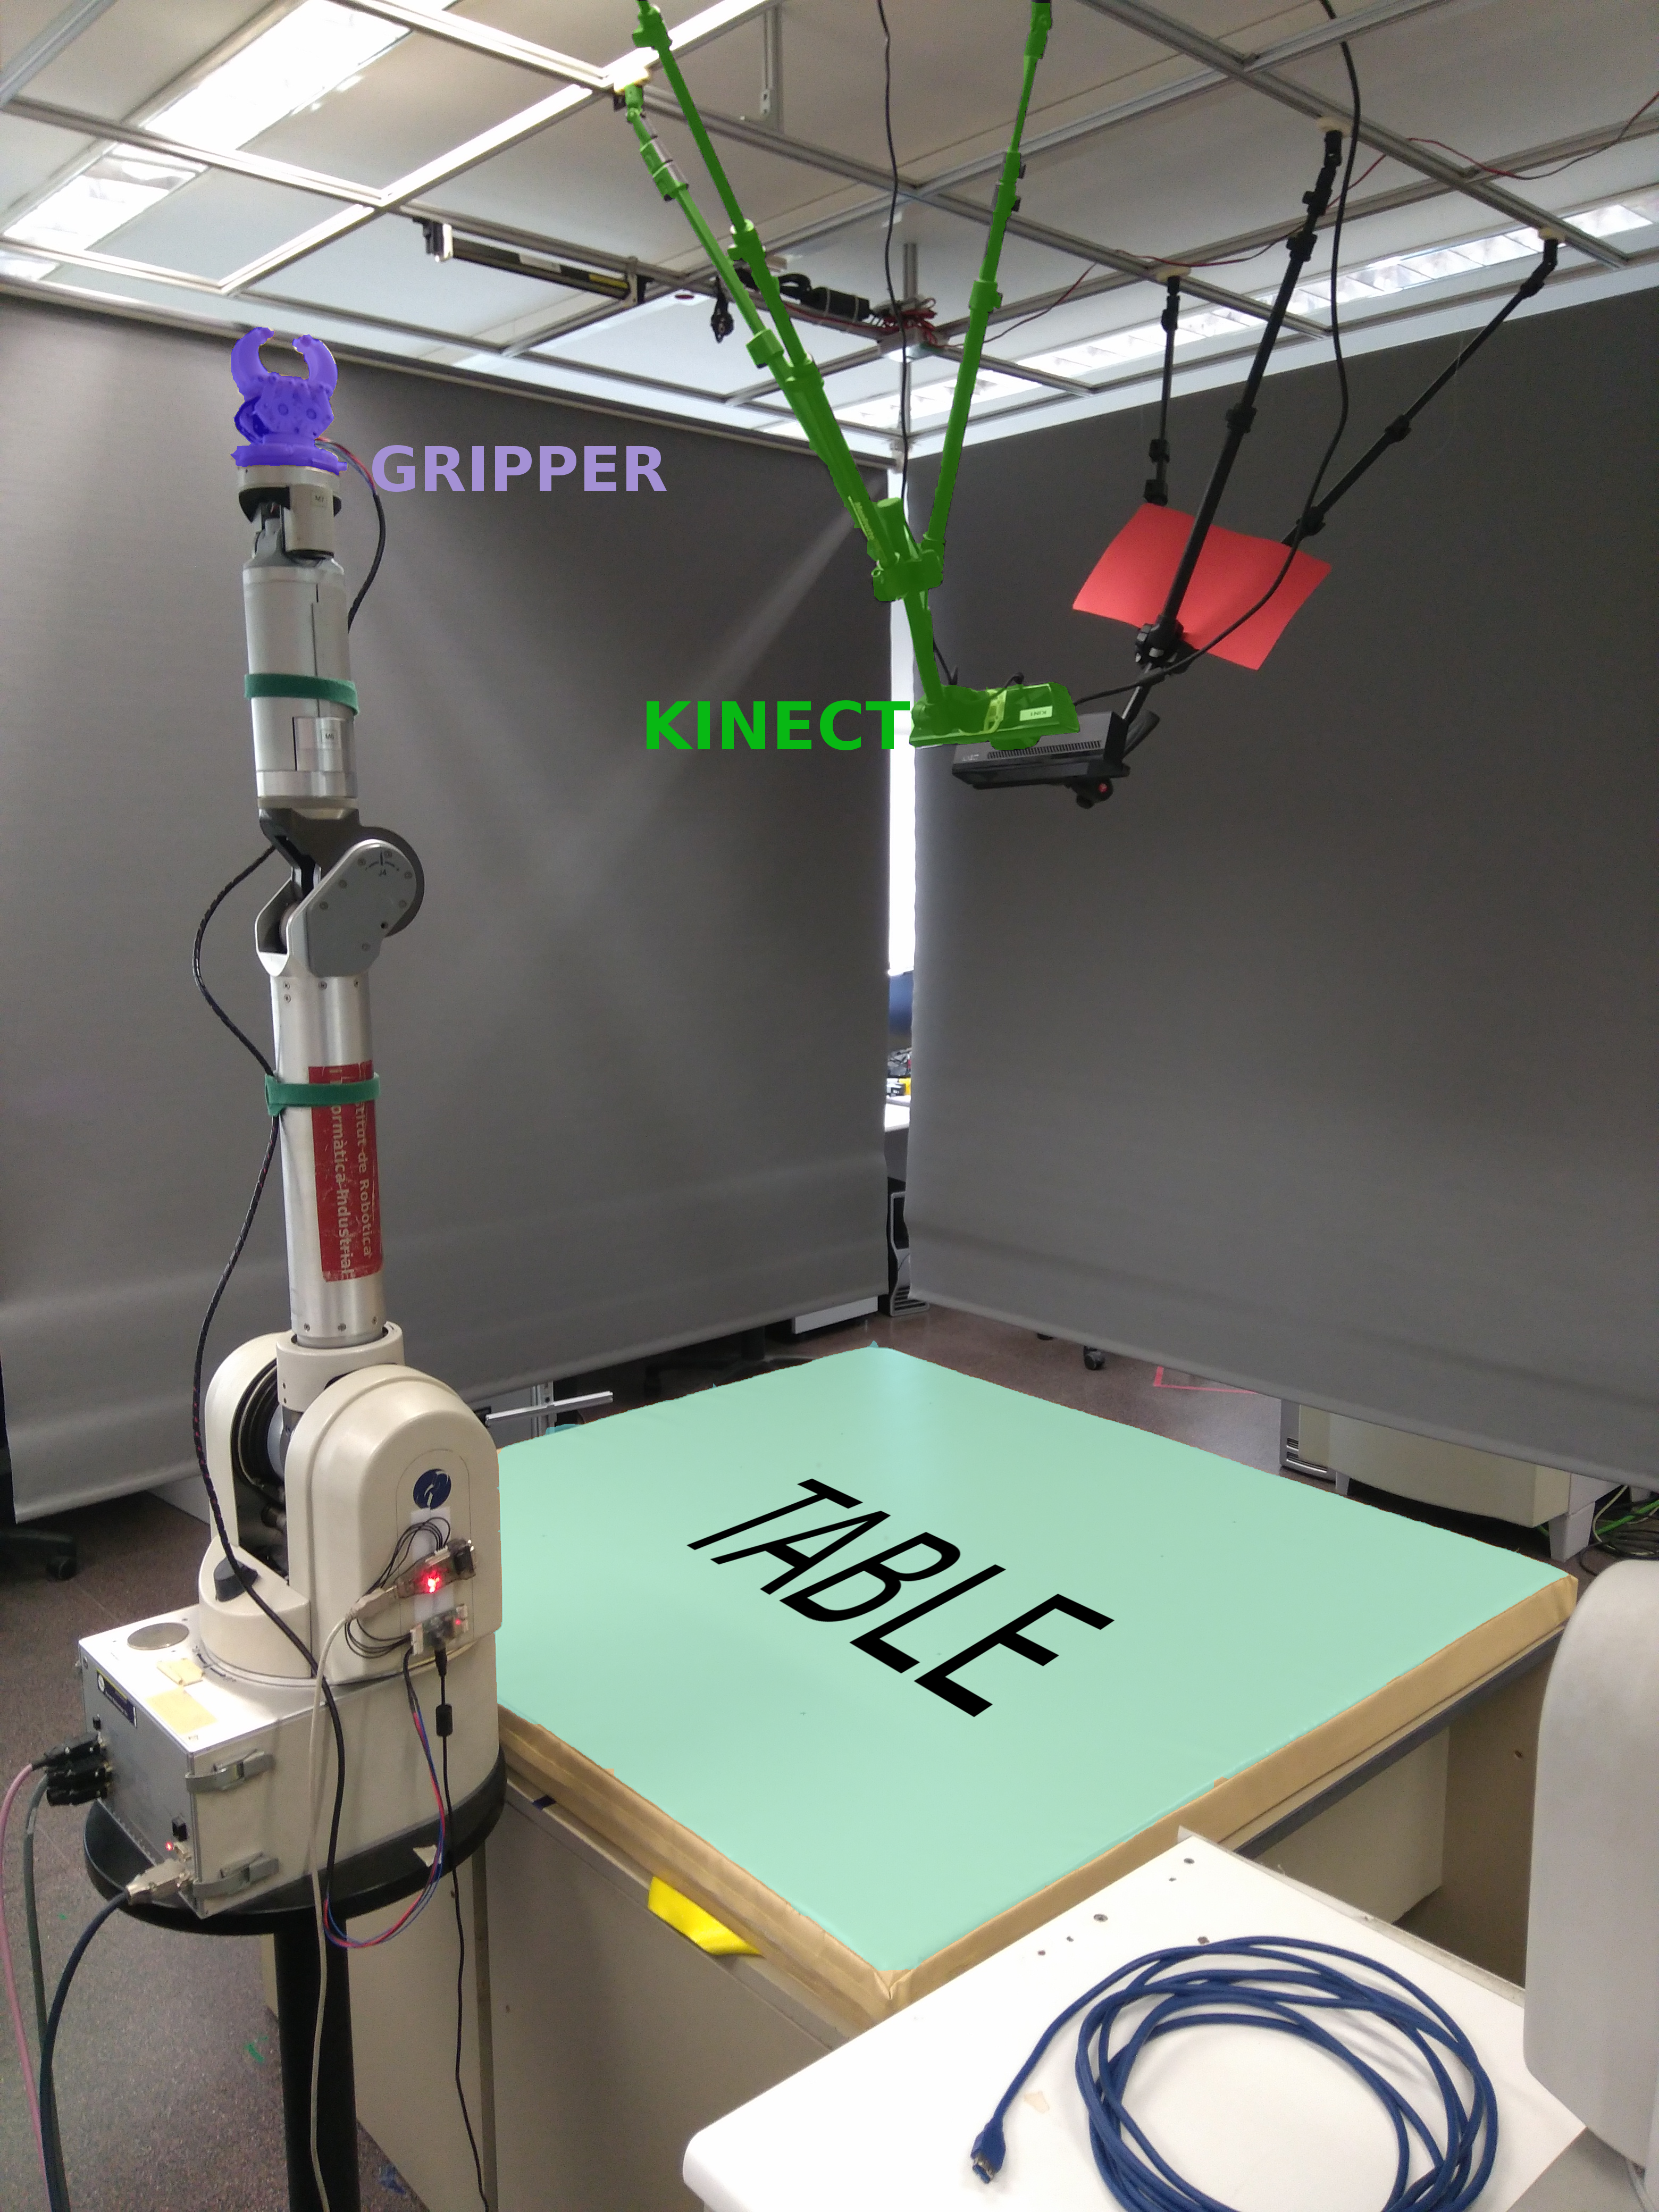
\includegraphics[height=9cm]{Img/set_up/set_up_nice.png}
\caption{Principal elements of the experimental set up.}\label{fig:setup_}
\end{subfigure}
\qquad \qquad 
\begin{subfigure}[b]{0.4\textwidth}
\centering
\includegraphics[height=4cm]{Img/set_up/example_setup.jpg}
\caption{Example of a cluttered scene the robot is going to work with.}\label{fig:example_scene}
\vspace{2ex}
\includegraphics[height=4cm]{Img/set_up/view_kinect.png}
\caption{Kinect's view.}\label{fig:kinect_view}
\end{subfigure}
\caption{Experimental set up, and example of a cluttered scene the robot is going to interact with.}
\label{fig:setup}
\end{figure}


Concerning the example of Figure \ref{fig:example_scene} it can be appreciate that the sequence of operation needed in order to clean all the table with a careful manipulation is quite complex, and due to the gripper geometry, and to the grasping poses we choose (section \ref{sec:grasping:pose}), the robot will need to grasp first the purple top object, or the white cup, then move one box in other to grasp the one of its side. All this sequence of actions will be decided by the robot.




\chapter{Previous works}
\label{ch:state_of_the_art}
In this chapter we present some previous works regarding manipulation planning. In the other chapters the state of the art will be introduced more in concrete accordingly to the chapter's topic.

Many manipulation planning approaches\citep{PlanningAlgorithms} assume that the task can be treated as a geometric problem with the goal to place the objects in their desired positions. Planning is essentially done with a mixture %\DMcomment{can you say mixture in this context?}
of symbolic and geometric states. They require to obtain the symbolic predicates that represent geometric features, which are very time consuming. Therefore, these hybrid planners can be too slow in real applications.  

%Such a symbolic predicates are hard to obtain and they could obtain by simulating the examples programs they learn the mapping from geometric states to symbolic states. Then a kernel density estimate is learnt from the training data of each predicate.
%In particular to the best of my knowledge, all the planners for cluttered scene are based on a mixture of symbolic and geometric predicates, or based only on geometric ones. 


Dogar and Srinivasa \cite{Dogar2011} proposed a framework for planning with cluttered scenes using a library of actions inspired by human strategies. They designed a planning system that decides which
objects to move, the order, where to move them, and the appropriate manipulation actions. Moreover, it accounts for the uncertainty
in the environment all through this process. 
The planning system first attempts to grasp the goal object, and if it is not possible, it identifies what is the object that prevents the action and adds it to a list of objects that have to be moved. Afterwards, those objects are moved in whatever position that makes the goal feasible. 
Their work is the most similar to our, but their planning system cannot be directly applied to a table clearing task. The goal is a single object at a time, then to grasp another object they need to replan. Our approach performs better with goals that involve more than one object. We plan sequence of actions considering all objects in the goal. The actions they use to move objects that were in the way may actually hinder future goals.
%Despite this, such a planning strategy can be used only in the design of a new planner, which is something we want to avoid.

%To grasp they used the Push-grasping action \cite{Dogar_2010_6652} , which is a robust way of grasping objects under uncertainty. It is a straight motion of the hand parallel to the pushing surface along a certain direction, followed by closing the fingers. For the pushing directions they used a resolution of $\pi/18$ rad (i.e. 36 different directions) and  use a predefined set of 9 hand aperture values. However their cluttered scenes is intended to be a scene with separated and well known objects. 

%In \cite{DBLP:conf/iros/SautGCSS10} they  don't use a manipulation planner, but just reduce the problem to motion planning and grasp planning.

% In \cite{DBLP:conf/iros/HaradaTNYOYK12} the authors propose an object placement planner for a grasped object during pick-and-place tasks. The proposed planner automatically determines the pose of an object stably placed near a user assigned point on an environment surface.

%In \citep{he.lahijanian2015towards-manipulation-planning} %(good place to stoole references :P in the introduction section) 
%the authors proposed to apply a linear temporal logic (LTL) planner to a manipulation planning task in cluttered scenes, but it suffers from poor runtime and the LTL specification is complex. Moreover to the scope of this work the temporal specification is not needed since it is indirectly encoded in the clutter scene composition. 

%\begin{displayquote}
%from the ABSTRACT:
%Robot manipulation is a challenging task for planning as it involves a mixture of symbolic planning and geometric planning. We would like to express goals and many action effects symbolically, for example specifying a goal such as for all x, if x is a cup, then x should be on the tray, but to accomplish this we may need to plan the geometry of fitting all the cups on the tray and how to grasp, move and release the cups to achieve that geometry. In the ideal case, this could be accomplished by a fully hybrid planner that alternates between geometric and symbolic reasoning to generate a solution. However, in practice this is very complex, and the full power of this approach may only be required for a small subset of problems. Instead, we plan completely symbolically, and then attempt to generate a geometric plan by translating the symoblic predicates into geometric relationships. We then execute this plan in simulation, and if it fails, we backtrack, first in geometric space, and then if necessary in symbolic. They assume the robot’s
%actions are reliable and that the world is perfectly known,and concentrate on the challenge of efficiently generating plans for these kinds of tasks (e.g. tidying a house).  It is clearly desirable to specify goals and reason at a symbolic level. 
%\end{displayquote}

%\begin{displayquote}
%We could create a classifier to classify the  the grasping %predicates. 
%\end{displayquote}


A recent alternative proposed by Mösenlechner and Beetz \citep{Msenlechner2009UsingPA} is to specify goals symbolically but evaluate the plan geometrically.
The idea is to use a high-fidelity physics simulation to predict the effects of actions and a hand-built mapping from geometric to symbolic states. Planning is conducted by a forward search, the effects of actions are determined by simulating them, and then the mapping is used to update the symbolic state. However, their method requires to know the physic of the manipulated objects to simulate them. Moreover the authors didn't test their planning system with a complex scene like the ones faced in this thesis.
Our planning system doesn't use any simulator, instead it relies on a prediction algorithm to represent how the objects can be manipulated, leading to a faster and easier to implement solution. 

%In \citep{lozano2014constraint}, Lonzano-Peréz et al. they use a simple task-level planner, in which operators are described with two types of preconditions: symbolic and geometric. They proposed a strategy for integrated task and motion planning based on performing a symbolic search for a sequence of high-level operations, such as pick, move and place, while postponing geometric decisions, based on the CSP (Constraint Satisfaction Problem) technique.


%Most methods ultimately involve a search at the task level in an abstract space, in which determining whether an operation is legal depends on the solution of a high-dimensional geometric motion-planning problem. Such approaches are particularly difficult to manage when a geometric decision made early in the high-level plan affects the feasibility of the rest of the plan in a way that is not revealed until later in the search. %An alternative approach is for the task-level planner to delay the binding of any geometric choices until it has constructed a plan "skeleton" that consists of unparameterized robot operations.  Note that in these constraint-based approaches, the geometric planner is in the inner loop of a symbolic planner, and must quickly decide whether a set of constraints is satisfiable.

%The solution they describe deterministically finds solutions for
%constraints in a quantized representation of the task parameters. The fidelity of the representation can be increased with a corresponding increase in computational cost. The use of a discrete representation allows us to use solution methods from the CSP (Constraint Satisfaction Problem). We use a simple task-level planner, in which operators are described with two types of preconditions: symbolic and geometric. Symbolic preconditions are described using symbolic fluents as is typical in symbolic planning formalisms. Whenever the symbolic search process reaches a state in which the symbolic aspects of the goal is satisfied, we extract a plan skeleton. A plan skeleton is accompanied by a set of constraints that relate the constraint variables that occur in
%the primitives. We call the CSP solver to see if the constraints associated with the plan skeleton are satisfiable.
% The correctness of a plan skeleton is enforced by the constraints, which are expressed as relationships between poses of objects in the world, poses of the robot hand, and configurations of the rest of the robot, as well as requirements that necessary clear paths exist.
% To formulate a domain as a discrete constraint satisfaction problem (CSP), it is necessary to specify: a set of constraint variables, a discrete domain of values for each variable, and a set of constraints. Constraints are specified by a set of variables to which they apply and an arbitrary test function that maps an assignment of variable values to True or False. One key advantage of a CSP formulation is that it reduces our job to picking variables and constraints to represent the problem, and uses a generic solver to do the search. It is generally easier to articulate and check constraints for a given assignment of the variables than to construct a problem-specific search strategy.
% The constraint-based formulation described here provides an attractive approach to integrating symbolic and geometric constraints for TAMP. One important drawback is the  need to pick an arbitrary discretization. 

%\textbf{In our context we are going to assume that the symbolic plans are feasible, instead to evaluate in a symbolic plan could also be geometrically feasible we manage the problem focusing on the scene interpretation in order to make the planner as simple as possible.}


%In \citep{stilman2007manipulation} the authors treat the problem of task planning in cluttered scene by working with only geometric relationships between objects.   

%In \citep{diankov2008manipulation} the authors presented a novel motion planning algorithm for performing constrained tasks. They addressed the problem of computing manipulation planning tasks such as grasping considering constraints of the object manipulated, so for example to open a door the robot have to consider the kinematic of itself and the one of the door. 


In \citep{coelhoplanning} the authors address a problem similar to the one of this thesis. The authors blended pushing and grasping actions for a table manipulation task.
%For pushing they used a similar strategy to \citep{mericli2013achievable}.
They use the concept of reachability \citep{vahrenkamp2013robot} to exclude impossible poses of the gripper at the planning stage, creating a reliable plan suitable for real-time operation. The authors model the planning problem through a Markov Decision Process (MDP), discretizing the world in grid cells and assigning each one a push and grasp vector defined by the reachability concept. Their advantage is that they plan a trajectory level so they can consider more details. In contrast, we plan at an action level, so we can consider more complex goals involving several objects, and will optimize the sequence of actions for completing the whole task.
% \DMcomment{Their advantage is that they plan a trajectory level so they can consider more details. In contrast, we plan at an action level, so we can consider more complex goals involving several objects, and will optimize the sequence of actions for completing the whole task (they only consider single-object tasks).}
%Our approach skips the modeling of the probability by considering to replan after each action execution, this eases our planning phase. \DMcomment{Don't talk about the replan in this case. Simply because probabilities are not useful for our case we don't replan, but maybe they are useful for their case as they plan at a lower level (trajectory level.)}
Moreover, while their method needs to be adapted to each robot, to build a reachability map, our method can be directly integrated in any robotic manipulator. 

%The world environment is composed of a table, objects placed on it and a gripper. The table surface is discretized in a fixed-sized grid. Each 3D cell is 3cm high. The width and length of the cells is established according to the dimensions of the table, so that all the table is covered by this discretization. Each cell is assigned with a pushability and a graspability vector. These two vectors translate the ability of the gripper to reach that cell in each one of the defined discrete orientations and then perform either a push or a grasp. Each cell is assigned with a pushability and a graspability vector. These two vectors translate the ability of the gripper to reach that cell in each one of the defined discrete orientations and then perform either a push or a grasp. To initialize the pushability and graspability vectors, the Inverse Kinematics at each cell is computed, with each one of the possible gripper’s orientation (72 values are defined). Then, for the pushability affordance, only if there is a path between the current pose and one on a fixed distance away along the direction of the tip, while maintaining the orientation of the gripper, will the corresponding entry in the pushability vector be set to true. Similarly, the graspability affordance on a certain pose is determined by computing a path from the current pose to one located a small distance up. If such a path exists, the graspability on that pose is set to true. For the objects they classify the objects accordingly to simple primivites shape. Their classification is done accordingly to the dimension of bounding boxes.	They assigned a reference frame for each object. It is not well specified which are the classes of objects considered.	They model the problem as a Markov Decision Problem. Having classified the object and consireding a finite set of possible discrete pose of the gripper with respect to the object it is easy performing the grasping. The nice thing of the MDP is that they model the pushing action, they have classified the object and for each discrete orientation considered they tried to perform the pushing action and learning in this way the transition model. Similarly for the grasping action. They use a RRT planner for the pushing action, given the initial and final object’s poses, the RRT algorithm explores the configuration space in order the get a path between these two poses. Modelled the transition model in this way they intrinsically know what is the best pushing direction, it is the planner that choose that.	
%The majority of the state of the art for task planning in cluttered scene is focused on designing a new planner, why in this thesis state of the art planners ready to use want to be used. 
%(If you want to talk more about this look the Related Work in \citep{abdo2013learning})
Symbolic planning requires knowledge about the preconditions and effects of the individual actions and such a knowledge can be obtained through machine learning techniques.
In \citep{abdo2013learning} the authors proposed an
approach to learn manipulation skills, including preconditions
and effects, based on teacher demonstrations.
%It is difficult to solve most real world manipulation tasks by reasoning purely in terms of low-level motions due to the high-dimensionality of the problems. Instead, robots should reason on a symbolic level and appropriately chain the learned actions to solve new tasks.  Such a planning step, however, requires knowledge of the important preconditions and effects of the actions.
With just a few demonstrations the method learns the preconditions and effects of actions. %Their method furthermore enables the robot to combine the learned actions by means of planning to solve new tasks that are more complicated than the learned individual actions. \DMcomment{I don't understand this last part}
This work looks promising since it allows to resolve planning problem by learning the model, but it is suitable only for simple actions. Having a hand-built model, like the one of our work, lets to resolve more complex problems and also it is more straightforward.

In \citep{Dearden2014355} Dearden and Burbridge proposed an approach for planning robotic manipulation tasks which uses a learned bidirectional mapping between geometric states and logical predicates. First, the mapping is applied to get the symbolic states and the planner plans symbolically, then the mapping is applied to generate geometric positions which are used to generate a path. If this process
fails they allow the system a limited amount of purely geometric backtracking before giving up and backtracking at the symbolic level to generate a different plan. However, this method cannot tackle complex scenes, such as cluttered objects, since in those cases learning a good mapping would be very hard.   
%\paragraph{Interpreting the scene}
%Focusing on symbolic planning, the research group of Artificial Intelligence and Robotics Laboratory of
%Istanbul Technical University, published some interesting researches suitable to the aim of this thesis. In \citep{ersen2014scene} \citep{SSS147762} \citep{ersen2013extracting} the authors propose a system which combines 3D recognition and segmentation results to create and maintain a consistent world model involving attributes of the objects and spatial relations among them. Unknown objects are modelled by using the segmentation output to determine their sizes and considering similarities with existing models to determine their shapes and colors. Then, these models are also stored as templates to be used for recognition along with the extracted attributes. 
%They focused on the extraction of size, shape and color attributes as well as the following unary and binary spatial relations: on, on ground/on table, clear and near for object manipulation scenarios. These predicates are generated and updated over time to maintain a consistent world model. 

Compared to the state of the art, we propose a planning system for clearing cluttered objects. Our approach plans at a symbolic level, which is efficient and is low time consuming  (the time to get a plan is usually less than $0.5$ seconds). As far as we know, previous approaches haven't tackled very cluttered scenes, such as the one in Figure \ref{fig:example_scene}. We will also show that the lack of geometric constraints introduces some limitations to the system, but the general results obtained are good and the planning phase is very efficient.  


%The \textit{on} relation for a pair of objects is determined by checking whether their projections on the table plane overlap. For each pair of objects the \textit{near} relation is determined by comparing the distance between the centers of these objects in each dimension with the sum of the corresponding sizes in that dimension. 

%About the \textit{on ground} predicate if the distance between the bottom surface of an object and the ground/table is observed to be within a certain threshold and no other objects can be detected under this object, it is determined to be on the ground or table. Surfaces are determined by plane 
%segmentation. \textbf{We can detect them like this: 1) bounding box 2) we compute the center of bounding box, if the distance from the center of it and the table plane is similar to its z dimension (along the table) up to a threhsold we can know if it is on the table or not - we can use it to speed up the calculation of \textit{on} predicate considering that only the objects that are not on the table can be on top on other ones.}



%%%%%% THE NEXT ARE COMMENTS (UNTIL THE END OF THE FILE)
\iffalse
\section{Usefull things}
Temporal filtering to reduce the noise of the kinect	 \citep{SSS147762}.

\section{Usefull Concepts}
 \textbf{Closed world} assumption \citep{Reiter87} can be defined
as having complete knowledge about the world, that is, the numbers and the attributes
of all objects are known apriori. 
\fi


\iffalse
\section{What we have}
\begin{itemize}
\item A naive pushing approach able to understand which object blocks the pushing action of another one.
For the pushing action we could try to create a classifier in order to understand what it is the most likely pushing direction using geometric features. In this case we can evaluate different directions and wwith the feasible ones we could choose the best one. 
To push we could use or ProMP or DMP. When we have more possible pushing directions choose the one the moves the nearer the center of the robot's workspace.
\textbf{Can we learn the pushing action? With a learning algorithm, not a classifier. Maybe we could create a classifier based on learning procedure.}
\item Understand when an object is on top of another one
\item Grasping? we miss how to decide if an object is graspable and if it is possible and, when it is not, understand if it is fault of an adjacent object. 
Strategy to resolve that:
\begin{itemize}
\item Haf algorithm (very expensive) first on the object considering adjacent objects and then only on the object, so we can compare and understand if that was feasible. 
\item HAF and then checking collision with the environment modelling in a simpler way the gripper, and detecting what are the objects that obstacle it

\textbf{With haf we also should test different rotations, this is too much expensive}
\item AGILE: (not too expensive, but still more or less 2-3 seconds for whatever point cloud) and it selects just randomly the grasping poses. It is not a good choice doing that except using a very large number of sample, in that case we also have to use a point cloud reconstruction to resolve the problems seen in my work. 
\item Naive approach: considering grasping it in the principal direction, it is computationally very cheap, and detecting for collision.
\item For objects that are not sorrounded by any other objects we should use a more powerfull algorithm in order to assure a good grasping pose detection.
\end{itemize} 
The most of state of the art dealing with problems similar to this one manage the grasping action as unfeasible for the part of object that obstacle the arm, not the gripper, since they are usually dealing with uncluttered scenarios, where the objects are all separated among themselves. The idea here is to relax the grasping checking in order to speed up the translation process into symbolic level. Then to perform real grasping a reliable algorithm is used in order to get a good grasping, and checked for collision. If it is not possible the grasping we can deduce that the robot is not able to find grasp it, and take off from the goal such object and all the objects. Considering the case that such an object is on top of another one also the bottom object cannot be included in the goal, so it should be not included into the planner's goal.
\end{itemize}
\fi





\chapter{Task planner}
\label{ch:task_planner}
In this chapter the general framework adopted is discussed, proposing a suitable task planner. After the  review of the current state of the art of task planners, a proper planner is chosen and then a suitable description to the table clearing problem is discussed.
\section{Task Planners Review}
As already seen in chapter \ref{ch:state_of_the_art} there exist different kind of planners and they can be grouped in three main categories:
\begin{enumerate}
\item classical planners
\item hierarchical planners
\item probabilistic planners
\end{enumerate}
\textbf{Classical planners}, as suggested by the name, are the more classical and easy to use. They are characterized by environments which are fully observable, deterministic, finite and static (changes happen only when the agent acts) and discrete (in time, actions, objects...) \citep{artificialIntelligence}.
A deterministic problem is generally formulated as a $6$-tuple $\Pi=\langle S^d, s_o^d, G^d, A^d, T^d, c^d \rangle$ \cite{little2007probabilistic}, where:
\begin{itemize}
\item $S^d$ is a finite set of states;
\item $s_o^d \in S^d$ is an initial state;
\item $G^d \in S^d$ is a goal state;
\item $A^d(s)$ is a set of applicable actions for each $s \in S^d$;
\item $T^d(a,s) \in S^d$ is a deterministic transition function for all actions $a \in A^d(s)$ and states $ s \in S^d$;
\item $c^d(a)$ is the cost to apply action $a$. 
\end{itemize}
The solutions, or trajectories, $\tau_i$ are sequences of actions applicable from the initial state until the goal state. The cost of a trajectory $C(\tau_i)$ is the sum of the cost of the actions of the trajectory $\sum_{a \in \tau} c^d(a)$. The optimal solution is the solution with less cost: $\tau^* = \min_{\tau_i} c(\tau_i)$. A very well known classic planner is the Fast Downward planner \cite{helmert2006fast}.

\textbf{Hierarchical planning}, also called \textit{Hierarchical Task Network}(HTN), works in a similar way to how it is believed that human planning 
works \citep{marthi2007angelic}. It is based on a reduction of the problem. The planner recursively decomposes tasks into subtasks, stopping when it reaches primitive tasks that can be performed directly by planning operators. This kind of planner needs to have a set of methods, where each method is a schema for decomposing a particular kind of task into a set of subtasks \citep{shopDescription}. For this kind of planning technique a well known planner is JSHOP2 \cite{JSHOP2}.

\textbf{Probabilistic planning} is a planning technique which consider that the environment is not deterministic but probabilistic. So the actions have a certain probability to obtain a certain state, and given an initial and final state the planner  finds the solution path with the highest probability. A well known example on which this kind of planners are build on is the Markov Decision Process. A probabilistic problem is generally formulated as a $6$-tuple $\Pi=\langle S, s_o, G, O, T, A \rangle$ \cite{little2007probabilistic}, where:
\begin{itemize}
\item $S$ is a finite set of states;
\item $s_o \in S$ is the initial state;
\item $G \in S$ is a goal state;
\item $O$ is the set of outcomes, the probability of $o \in O$ is $Pr(o)$;
\item $T(o,s) \in S$ is a (total) deterministic transition function for all outcomes $o \in O$ and states $s\in S$;
\item $A(s)$ is a set of applicable actions for each $s \in S$, coupled to a function $out(a) \subseteq O$ mapping each action to a set of outcomes in such a way that 
\begin{itemize}
\item each outcome $o \in O$ belongs exactly to one action $act(o)$;
\item $\sum_{o \in out(a)} Pr(o) = 1$ for all $a$.
\end{itemize}
\end{itemize}
In this case the optimal solution is the one with the highest probability. In this category two famous probabilistic planners are Gourmand \cite{Gourmand} and PROST \cite{PROST}.

\section{Planner}
The problem this thesis is facing could be resolved by several approaches by using planners from all the categories. We have already seen that such a problem involves geometric constraints and those cannot be considered directly by the planner using a ready to use state of the art planner, that would imply a designing of a new planner. Moreover using a hybrid planner is also time consuming, so we decided to focuse on a strategy that would let us to use already existing planners. This way involves working with symbolic predicates. Symbolic predicates are predicates which can be true or false, and they will be introduced more in detail in the next sections. 

The problem moreover involves a big amount of uncertainty due to the interaction of the robot with the environment. When the robot will interact with the objects it is very hard to predict correctly the position of the object in the next frame, that is the next state, this is a crucial problem which should be considered. With a probabilistic planner, the planner will take into account what object has been moved and it will update the state obtaining a set of states, each one with a certain probability, and the returned plan, or solution, is the one with the highest probability. The probability also has to be modelled and it is highly depending on the form of the object, this makes the modelling of the probability a problem.
Martinez et al. \citep{martinez2015planning} faced the problem of cleaning a surface entirely by probabilistic symbolic planning. The problem they wanted to solve was characterized by a strong probability and a wrong effect of the action would have lead to replan and therefore to slow down the system.
Another way to face the problem is to replan at each frame, that is after each interaction of the robot with the pile of objects, or whenever the current state deviates from the expected one, generating a new trajectory from the current state to the goal. The plan's actions are considered deterministic, and the only useful action is actually the first one of the plan, after its execution the system replans again. Little et al. discussed in \cite{little2007probabilistic} the problem of when is more useful the probabilistic planning with respect a simple replanning system. 
They defined a the concept of \textit{Probabilistic Interesting Problem} with the following definition:

\begin{displayquote}
A probabilistic planning problem is considered to be \textit{probabilistically interesting} if and only if it has all of the following structural properties:
\begin{itemize}
\item there are multiple goal trajectories;
\item there is at least one pair of distinct goal trajectories, $\tau$
and $\tau'$, that share a common sequence of outcomes for the
first $n-1$ outcomes, and where $\tau_n$ and $\tau_n'$ are distinct
outcomes of the same action; and
\item there exist two distinct goal trajectories $\tau$ and $\tau'$ and outcomes $o \in \tau$ and $o' \in \tau'$ of two distinct actions $a = act(o)$ and $a' = act(o')$  such that executing action $a$ strictly decreases
the maximum probability of reaching a state where action $a'$ can
be executed. To clarify: executing $a$ rules out any plan with a maximal probability of executing $a'$.
\end{itemize}
\end{displayquote}
They assert that unless a probabilistic planning problem satisfies all of the structural conditions in this definition, then
it is inevitable that a well-written replanner will outperform
a well-written probabilistic planner. Moreover the authors do not negate the possibility that a deterministic replanner could perform optimally even for probabilistically interesting planning problems. 

To conclude, a replanner would make more probabilistic problem practically solvable. In the other hand it suffers to be less robust than a probabilistic one. 


\begin{comment}
From their analysis the state that probabilist planning has some useful properties which a deterministic replanning does not have, and they are:
\begin{itemize}
\item The lack off \textit{dead end} states, from which the goal is unreachable through any
combination of chance and choice,
\item  the degree to which the probability of reaching a \textit{dead end} state can be reduced through the choice of actions,
\item a higher degree in the solution trajectory, yielding to possible several and feasible solutions,
\item  the presence of mutual exclusion
\end{itemize}
\end{comment}

Taking into account such considerations, in order to face simply such a difficult problem, the problem has been thought to be solved thanks to a deterministic replanner although it is \textit{probabilistic interesting}. The choice also was guided by the difficulty to model the probability distribution of the actions which depends on the particular shape of the objects the robot has to interact with. 

Between a classic planner and an heuristic one there is not much difference for the aim of this work.
The planner chosen to develop the work is the \textbf{Fast Downward} planner \cite{helmert2006fast}\cite{FastDownwardPage}, a very well know classic one. The advantage of this planner is its wide documentation with respect other planners, which makes it easier to use and it also has a wide community. 

\section{Symbolic Predicates}
One the planner has been chosen, the planning problem has to be formulated accordingly to the capabilities of such a planner. The \textit{Fast Downward} planner needs the problem to be formulated in the common format of PDDL (\textit{Problem Domain Description Language}) \citep{pddl}. In this section the symbolic predicates that have been considered in order to resolve the problem are described.

The task this thesis is going to resolve is a common task done by humans who thinks in order to find a feasible sequence of actions. Such a sequence is normally composed of actions that avoid the collision between the manipulated object and the other ones, whenever possible. To do this we, as human, think on what is going to happen if we manipulate an object in a certain way, and what objects can be manipulated at the current instant and what objects need to be moved in order to interact with a certain one. The design of the problem has been inspired on such a reasoning way. The reasoning part is entrusted to the planner, which needs a coherent problem description through symbolic predicates. 

How described in the introduction, the system will be able to perform two types of actions: \textbf{pushing} and \textbf{grasping}.
Grasping action is a necessary action in order to grasp an object and drop it into a bin, while the pushing action is an auxiliary action which has the aim to move an object in order to collocate it in a pose that do not obstacle the solution of the plan. In fact it happens that an object cannot be grasped because there is an adjacent one that impedes such an action.
The pushing action is said to be an auxiliary because it is not strictly necessary to solve every kind of problem, depending on the cluttered scene the grasping action could be enough.
The coupling of these two actions makes wider the range of problem this planner can solve.    

The symbolic predicates are designed accordingly to the available actions trying to answer the following questions:
\begin{itemize}
\item When cannot an object be grasped? 
\item When can a object be pushed? In which direction? 
\end{itemize}

\paragraph{Grasping Action}
An object cannot be grasped always but only if the grasping action is not impeded by other objects, to do this we need to check that:
\begin{itemize}
\item no objects stand on top of the interested one
\item there are no adjacent objects that imped the grasping action
\end{itemize}
We don't want to grasp an object which has another one on top of it for one main reason: during the grasping action the top object will fall corrupting the scene and such behaviour is undesired, in fact an human will never grab an object at the bottom of another one without first grabbing the one on the top. To include such an information in the problem description the predicate \textbf{on} is created, in particular it is defined as \texttt{(on o1 o2)} meaning that object labelled as \texttt{o1} stands on top of \texttt{o2}.

Once we are sure the current object has no objects on top of it we have to check if it can be grasped, that is, given a grasping pose we have to check if that pose is feasible or if it is impeded by other objects. To include such an information in the problem description the predicate \textbf{block\_grasp} is created. In particular it is defined as \texttt{(block\_grasp o1 o2)} meaning that object labelled as \texttt{o1} impedes object \texttt{o2} to be grabbed.

\paragraph{Pushing Action}
In certain situations when the grasping is not possible because an object impedes another one to be grasped one of them has to be moved, otherwise the problem has no solution. Firstly, being observant of the philosophy to avoid manipulation that can damage the objects, we considered that only the objects that stands on the table can be pushed, that is an object on top of another one will be no pushed. And, how discussed for the grasping action, also an object that has on top of itself another one will be no pushed.
Second, the possible directions along with an object can be moved have to be decided. Such directions are taken accordingly to the shape of the object, in particular to its principal axis (see Section \ref{sec:background_alg}). From the principal axis we are able to find 4 possible pushing directions per object. To the best of my knowledge there are no studies about how pushing an object on a proper way, or direction, in order to make it follow a desired trajectory. 

Having the direction each object can be pushed along with, the next step is to understand if the object can be pushed along those directions. An object cannot be pushed in a certain direction if there is another one that blocks the current object. For each direction the object is therefore translated in the pushing direction and checked for collision with other objects. In this way it is possible to get what is the object which impedes the considered one to be moved along the considered direction. 

To include such an information the predicates \textbf{block\_dir1}, \textbf{block\_dir2}, \textbf{block\_dir3} and \textbf{block\_dir4} are created. In particular, they are defined as \texttt{(block\_dir}$_i$\texttt{ o1 o2)} meaning that the object labelled as \texttt{o1} is impeding object \texttt{o2} to be moved along direction \texttt{dir}$_i$.

\paragraph{Effects of the actions}
The effects of the action has to change the current predicates of the problem in order to update coherently the state. For the \textit{grasping} action whenever an object is grasped, since we are working in a deterministic scenario, the object is supposed to be grasped successfully and drop in the bin. If such an object was on top of other ones, it was impeding some objects to be pushed in some direction or to be grasped those predicates have to be update coherently. Moreover to considered that the object is no more in the scene the predicate \textbf{grasped} is added. In particular \texttt{(grasped o1)} means that the object labelled as \texttt{o1} has been grasped and dropped into the bin, and therefore there is nothing more to do with it. The \textit{pushing} action, still thinking in a deterministic scenario, is supposed to be done in a manner that the object will be moved far enough from the others in such a way that it can be considered isolated. Considering it is isolated from the others, if it was blocking some object to be pushed in a certain direction now it will not impedes no more, and the same if an object impeded the current one, so the \texttt{block\_dir}$_i$ predicates are update, and the \texttt{block\_grasp} as well.  

	
\paragraph{Geometric constraints}
The proposed planner until now does not include any geometric information, such as whether the robot can actually perform a certain action. It may happens that the object is outside the working space of the robot and this makes it hard to interact with. In such a case the robot will have a plan but it is impossible its execution, this make the plan unfeasible. 

This aspect has to be taken into account and it can be done using a common technique in task planning such as \textbf{backtracking} \citep{Bidot2015}. The backtracking technique is about compensating the gap between planning with abstract actions and some physical and geometric constraints such as kinematics. Backtracking is based on updating the initial state used to get the current plan considering the geometric and kinematics constraints, and replan again with the updated initial state, obtaining in this way a different plan that could be feasible. The obtained plan will still be evaluated and backtracked until a feasible plan is obtained or there exists no plan. The pseudo algorithm is shown in Algorithm \ref{alg:backtracking}.

\begin{algorithm}
\caption{Planning procedure with backtracking. The input parameters are the initial state and the goal state. Given a plan, an action is defined by the kind of action and the object of interest ($action, object$). The procedure will return a feasible plan or not plan at all.}\label{alg:backtracking}
\begin{algorithmic}
\Procedure{GetPlan}{$state_{init}$,$goal$}
\Repeat
  \State $plan =$ \textsc{GetFastDownwardPlan}($state_{init}$,$goal$)
  \If{\textsc{isPlanEmpty}()} 
  		\Return NULL 
  \EndIf
  \State $action, object =$ \textsc{GetFirstAction}($plan$)
  \State $success =$ \textsc{HasIKSolution}($action, object$) 
  \If{$\neg success$}
    \State $state_{init} =$ \textsc{UpdateInitialState}($action, object$) 
  \EndIf
\Until{$success$}
\Return $plan$
\EndProcedure
\end{algorithmic}
\end{algorithm}  

This technique is a very common technique for planners that plans symbolically and have no informations about geometric constraints. This is considerable limitation of symbolic planning but since they are typically very fast to execute, backtracking and replanning will not make them to much slower.

Let's consider to include the geometric information, such as path planning or inverse kinematics, into the geometric planner. The inverse kinematics by itself is an expensive operation, overall considering the high degree of freedom of the WAM arm. The most of the times the objects are considered to lie inside the working space of the robot. Computing the inverse of Kinematics for each possible action for each object would be very expensive, and by experimental result we can say that the majority of the times the inverse kinematics is feasible and the majority of the plans are also feasible. Moreover, due to the probability of the next states the planner has to replan at each frame, and computing the predicates means computing the inverse kinematics as well. All this would make the planner process extremely time consuming when it is not needed. Path planning is even more computational costly than the inverse kinematic. 
  
To consider the geometric unfeasibility of an action a predicate for each action is added: \ttt{(ik\_unfeasible\_dir1 ?o)},  \ttt{(ik\_unfeasible\_dir2 ?o)},  \ttt{(ik\_unfeasible\_dir3 ?o)}, \linebreak \ttt{(ik\_unfeasible\_dir4 ?o)} and  \ttt{(ik\_unfeasible\_grasp ?o)}. The backtracking procedure will try to execute the action by first computing a solution for the inverse kinematic for the path to execute, the pushing action will be a sequence of points in the Cartesian space and the grasping action will be composed of a pre-grasping pose and a grasping pose. If the first plan's action on a particular object is not possible to execute one of those predicates is added. 

It is possible that an object cannot be grasped on a certain pose but it can be moved in a new pose in which it can be grasped. Therefore the pushing actions also will include the effect that the object of interest will have a solution in the inverse kinematic for the new pose. This is usually a rare case but it might happen. Of course, since the planner has no geometric information, it does not know in which pushing direction the object can be reach a position where it can be grasped, therefore this will be a totally random choice up to the planner. In the case the object is in a pose where it cannot be neither grasped or pushed because of the inverse kinematic, first the planner will return as a solution to grasp it, then it will replan and the solution will be to push it in one direction and grasp it, and so until no action can be executed and there exist no solution for the plan. In the best case, the planner will chose to push the object in direction in which the next pose will be more likely a graspable one. 


\todo[]{Include this in the experiments?}
\begin{figure}[h]
\centering
\includegraphics[width=5cm]{Img/backtracking/image4.png}
\caption{Unfeasible plan due to geometric constraints. In this case the planner returns as action to execute grasping or pushing away the white cup (highlighted by a red circle) but it is out the configuration space of the robot and there exist no plan for that problem. This problem is the one depicted in Figure \ref{fig:example_scene}, where the other objects has been grasped as consequence of the plan execution.} \label{fig:backtracking1}
\end{figure}

A situation in which the backtracking is useful is shown in Figure \ref{fig:backtracking1}. Accordingly to our strategy, the robot cannot be grasp the black or red box because the gripper would collide, and the same for the pushing action. It has to interact with the white cup in order to make space to move the other objects and then grasp them. The planner first returns the following plan: \texttt{(grasp o2)}, \texttt{(push\_dir1 o0)}, \texttt{(grasp o1)}, \texttt{(grasp o0)}. It will try to solve the inverse kinematic for the \texttt{(grasp o2)} action, but it found no solutions. Therefore the predicate \ttt{(ik\_unfeasible\_grasp o2)} is added and the planner replans. The new plan is: \texttt{(push\_dir1 o2)}, \texttt{(grasp o2)}, \texttt{(push\_dir1 o0)}, \texttt{(grasp o1)}, \texttt{(grasp o0)}. In this case it will try to get a solution for the inverse kinematic for the pushing action but it finds no solution, so the predicate \ttt{(ik\_unfeasible\_dir1 o2)} is added. And so on until the planner finds that all the possible actions for a feasible plan have no solutions for the inverse kinematic. In this way the planner includes the ability to understand also why there exist no plan for a certain problem. 

It may happen that the object outside the working space of the robot blocks the execution of the task because if the planner insists to return as first action an action with that object, then it will find that is not possible to interact with it and therefore there exist no solution on the planner procedure, this is the case previously presented. 
To overcome this, problem, and make the problematic objects left as the last one to interact with if possible, the actions are enhanced with another effect, that is all the objects that have one of the unfeasible inverse kinematic predicates set to true, are set to false. In this way, if possible, only the first action considers the geometric constraints, while the next ones have no information about the geometric constraints. 

\paragraph{PDDL}
For clarity purposes, the PDDL syntax of the described action is here reported. 
For the \textit{grasping} action its PDDL syntax is shown in listing \ref{graspPDDL}.

\lstset{language=pddl}
\begin{lstlisting}[caption={PDDL syntax of the grasping action},label=graspPDDL]
(:action grasp
    :parameters (?o - obj)
    :precondition (and
                  ; grasp it if there are no objects on its top
                  (not (exists (?x - obj)(on ?x ?o)))
                  ; grasp it if there is no object that blocks it
                  ; to be grasped
                  (not (exists (?x - obj)(block_grasp ?x ?o))))
    :effect (and
            ; the object "o" is grasped
            (grasped ?o)
            ; if the object was on top of other ones now it is
            ; no more on top of them
            (forall (?x - obj)
              (when (on ?o ?x) (not (on ?o ?x))))
            ; the grasped objects no more blocks other objects 
            ; to be pushed or grasped
            (forall (?x - obj)
              (when (block_grasp ?o ?x) (not (block_grasp ?o ?x))))
            (forall (?x - obj)
              (and
              (when (block_dir1 ?o ?x) (not (block_dir1 ?o ?x)))
              (when (block_dir2 ?o ?x) (not (block_dir2 ?o ?x)))
              (when (block_dir3 ?o ?x) (not (block_dir3 ?o ?x)))
              (when (block_dir4 ?o ?x) (not (block_dir4 ?o ?x))))
              ; remove all geometric constraints 
              (when (ik_unfeasible_dir1 ?x)(not (ik_unfeasible_dir1 ?x)))
              (when (ik_unfeasible_dir2 ?x)(not (ik_unfeasible_dir2 ?x)))
              (when (ik_unfeasible_dir3 ?x)(not (ik_unfeasible_dir3 ?x)))
              (when (ik_unfeasible_dir4 ?x)(not (ik_unfeasible_dir4 ?x)))
              (when (ik_unfeasible_grasp ?x)(not (ik_unfeasible_grasp ?x))))))
\end{lstlisting}

For the \textit{pushing} action its PDDL syntax is shown in listing \ref{pushPDDL}.

\lstset{language=pddl}
\begin{lstlisting}[caption={PDDL syntax of the pushing action along direction 1},label=pushPDDL]
(:action push_dir1
    :parameters (?o - obj)
    :precondition (and
                  ; push in direction 1 only if there are no
                  ; objects that block it along that direction
                  (not (exists (?x - obj)(block_dir1 ?x ?o)))
                  ; push it if it has no objects on top of it
                  ; and if it not on top of other ones
                  (not (exists (?x - obj)(on ?x ?o)))
                  (not (exists (?x - obj)(on ?o ?x))))
    :effect  (forall (?x - obj)
               (and
               ; once pushed the object is no more blocked in any direction
               ; and it no more blocks other objects to be moved
               (when (block_dir1 ?o ?x) (not (block_dir1 ?o ?x)))
               (when (block_dir2 ?o ?x) (not (block_dir2 ?o ?x)))
               (when (block_dir3 ?o ?x) (not (block_dir3 ?o ?x)))
               (when (block_dir4 ?o ?x) (not (block_dir4 ?o ?x)))
               (when (block_dir1 ?x ?o) (not (block_dir1 ?x ?o)))
               (when (block_dir2 ?x ?o) (not (block_dir2 ?x ?o)))
               (when (block_dir3 ?x ?o) (not (block_dir3 ?x ?o)))
               (when (block_dir4 ?x ?o) (not (block_dir4 ?x ?o)))
               ; once pushed it can be grasped and it no more
               ; blocks other objects to be grasped
               (when (block_grasp ?x ?o) (not (block_grasp ?x ?o)))
               (when (block_grasp ?o ?x) (not (block_grasp ?o ?x))))
               ; remove all geometric constraints 
               (when (ik_unfeasible_dir1 ?x)(not (ik_unfeasible_dir1 ?x)))
               (when (ik_unfeasible_dir2 ?x)(not (ik_unfeasible_dir2 ?x)))
               (when (ik_unfeasible_dir3 ?x)(not (ik_unfeasible_dir3 ?x)))
               (when (ik_unfeasible_dir4 ?x)(not (ik_unfeasible_dir4 ?x)))
               (when (ik_unfeasible_grasp ?x)(not (ik_unfeasible_grasp ?x)))))
\end{lstlisting}

\mbox{}


With such predicates the planner has all the basic information about the location of the objects on the scene. The symbolic predicates try to simplify the problem translating the geometric properties of the objects in symbolic ones. It is important to point out again that the system is deterministic, meaning that all the actions are supposed to give the resultant state with a probability of $1$. Clearly the more uncertainty is related to the pushing action, the direction selection, based on the principal axis, does not taken into account reliably the geometry of the object. The trajectory will be unlikely the desired one but a similar one. Overall the planner is considering to push the objects at infinity to isolate it, and that's false. This is another uncertainty of the pushing action due to the lack of geometric information. 
After the execution of an action the planner gets a new depth image from the Kinect, it segments the scene, it recomputes the predicates and replans. In this way the planner considers a totally new problem and all the uncertainties associated to the previous plan will be resolved to the current one. 
%In this manner we are forced to considered that some interactions between objects are allowed but tried to be avoid as much as possible. 

In order to provide a graphical scheme to the reader the planner pipeline is depicted in Figure \ref{fig:pipeline}. It can be appreciated the two fold strategy of the algorithm, the first stage (Figure \ref{fig:pipeline1}) is devoted to get the predicates from the Kinect sensor and the second one to evaluate the feasibility of the returned planned through backtracking and to execute the plan(Figure \ref{fig:pipeline2}).

\begin{figure}[t]
\centering
\begin{subfigure}[t]{\textwidth}
\centering
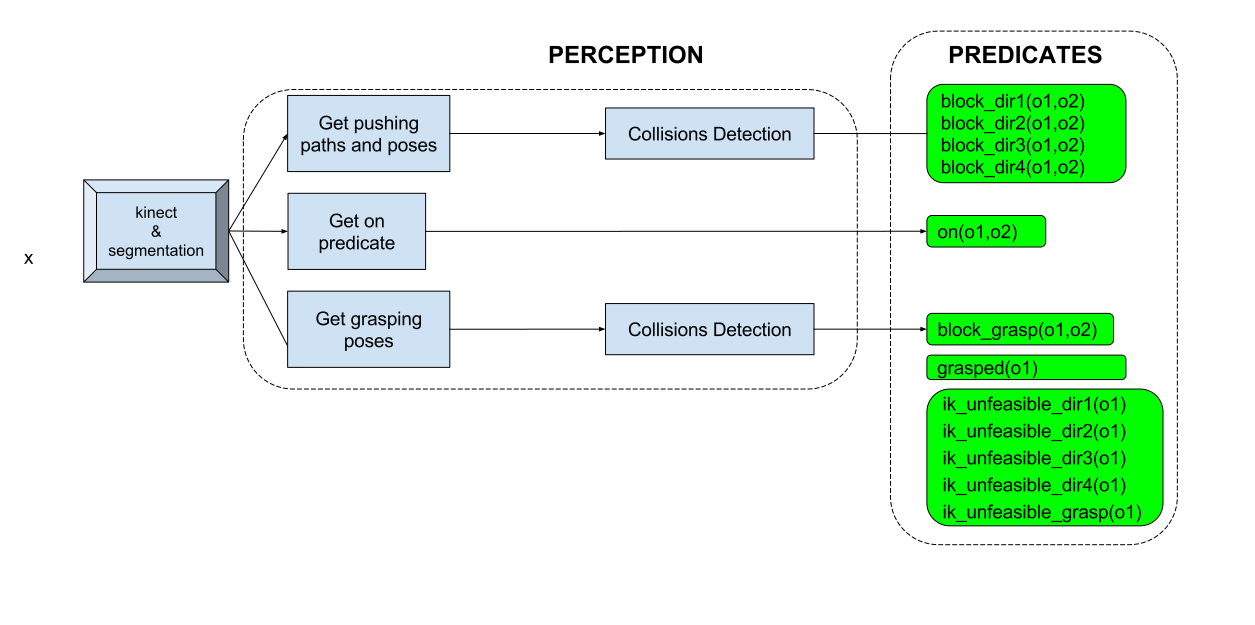
\includegraphics[width=\textwidth]{Img/planning/Pipeline1.png}
\caption{Perception Pipeline}\label{fig:pipeline1}
\end{subfigure}
\begin{subfigure}[t]{\textwidth}
\centering
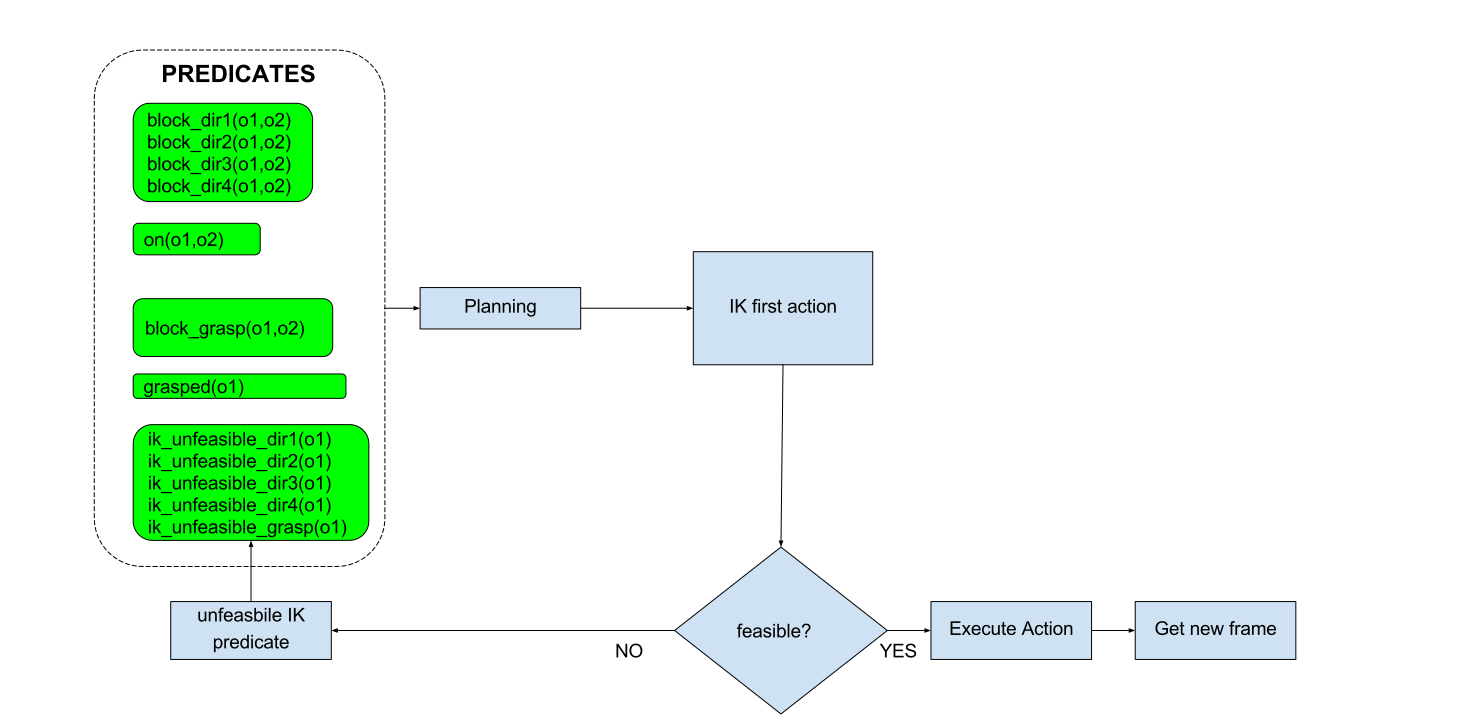
\includegraphics[width=0.9\textwidth]{Img/planning/Pipeline2.png}
\caption{Planning Pipeline}\label{fig:pipeline2}
\end{subfigure}
\caption{Planner pipeline}\label{fig:pipeline}
\end{figure}

Notice that the \ttt{grasped} predicate is just a predicate used only by the planner in order to know when the object has reached the goal or not, it does not need to be updated by the task planner. 

\mbox{}

How the predicates are computed will be discussed in detail in the next chapter.




\chapter{Implementation}
\label{ch:implementation}

In this chapter the implementation is discussed, presenting how the objects are recognized and how the symbolic predicates are obtained. 

\section{Object Localization} 
For the planner, to know how to move the object, is fundamental knowing the objects on the scenario, therefore they need to be detected. More correctly, they need to be segmented since the algorithm is dealing with unknown objects, it is not going to recognize an objects as a particular one, but it segments the objects. 

This stage is composed on two steps:
\begin{enumerate}
\item Detecting the table top objects
\item Segmenting the table top objects
\end{enumerate}
The depth sensor is recording a depth map of a table, the algorithm has therefore to detect first the table, and so the objects that stands on top of it, and then segmenting them. We don't want to segment the entire image, if so, the table will be segmented as an object and the floor as well.

\subsection{Tabletop Object Detection} 
The strategy for the tabletop object detection phase is composed of 3 different steps:
\begin{enumerate}
\item \textbf{Table plane estimation} (by RANSAC): the points of the table are detected estimating first a plane in the point cloud, all the points which belong to such a plane are the points of the table. 
\item \textbf{2D Convex Hull of the table}: having the points of the table a 2D convex hull is computed in order to get a 2D shape containing those points.
\item \textbf{Polygonal prism projection}: all the points are projected on the table plane previously estimated and all the points which projections belong to the 2D convex hull are considered to be points of tabletop objects. 
\end{enumerate}

\begin{figure}[htp]
\centering
\begin{subfigure}[t]{0.32\textwidth}
\includegraphics[width = 1.1\textwidth]{Img/ObjectSegmentation/pcl.png}
\caption{Input Point Cloud}\label{img:obj_pointcloud}
\end{subfigure}
\begin{subfigure}[t]{0.32\textwidth}
\includegraphics[width = 1.1\textwidth]{Img/ObjectSegmentation/ransac.png}
\caption{RANSAC plane estimation}\label{img:obj_ransac}
\end{subfigure}
\begin{subfigure}[t]{0.32\textwidth}
\includegraphics[width = 1.1\textwidth]{Img/ObjectSegmentation/plane.png}
\caption{Table plane}\label{img:obj_plane}
\end{subfigure}
\begin{subfigure}[t]{0.32\textwidth}
\includegraphics[width = 1.1\textwidth]{Img/ObjectSegmentation/convex_hull.png}
\caption{Convex Hull}\label{img:obj_conex_hull}
\end{subfigure}
\begin{subfigure}[t]{0.32\textwidth}
\includegraphics[width = 1.1\textwidth]{Img/ObjectSegmentation/convex_hull_full.png}
\caption{Convex hull in the point cloud}\label{img:obj_convex_hull_full}
\end{subfigure}
\begin{subfigure}[t]{0.32\textwidth}
\includegraphics[width = 1.1\textwidth]{Img/ObjectSegmentation/tabletop_objects.png}
\caption{Tabletop objects}\label{img:obj_tabletop_objects_results}
\end{subfigure}
\caption{\textbf{Object Segmentation:} Given the point cloud (\subref{img:obj_pointcloud}), the estimated table's plane is obtained (\subref{img:obj_ransac} and \subref{img:obj_plane}), its convex hull is extracted (\subref{img:obj_conex_hull} and \subref{img:obj_convex_hull_full}), and the tabletop objects are obtained by a polygonal prism projection (\subref{img:obj_tabletop_objects_results}).}
\label{img:obj_tabletop_objects}
\end{figure}

The steps of this tabletop object detection algorithm are described in Figure \ref{img:obj_tabletop_objects}   for the point cloud\footnote{Point cloud taken from the Object Segmentation Database (OSD) \href{http://users.acin.tuwien.ac.at/arichtsfeld/?site=4}{http://users.acin.tuwien.ac.at/arichtsfeld/?site=4}} in Figure \ref{img:obj_pointcloud}.

\subsection{Object Segmentation}
\label{sec:obj_seg}
Once the objects on the table are detected the following phase is to segment them in order to get a point cloud per object.

\subsubsection{Supervoxel}

For their segmentation the supervoxel concept is used. A supervoxel is a group of voxels that share similar characteristics. 
%and it is equivalent to the superpixel concept for the voxel case. Superpixel is a widely used preprocessing step in segmentation
%algorithms  which allows to reduce the number of regions
%that must be considered later by more computationally
%expensive algorithms, with a minimal loss of information. 
%The supervoxel concept is the extension of the superpixel method to the point clouds. A voxel represents a single sample on a regularly spaced, three-dimensional grid. A supervoxel 

In this work the supervoxels are computed with the Voxel Cloud Connectivy Segmentation (\texttt{VCCS}) algorithm \cite{Papon13CVPR}, which was proposed in 2014 and gives good improvements with respect to previous state of the art methods, and still it is able to be used in online applications. 

The algorithm works in 4 main steps:
\begin{itemize}
\item Voxelizing the point cloud
\item Creating an adjacency graph for the voxel-cloud 
\item Creating seeds for the initial supervoxels centres
\item Each seed is described by $39$ features that describe spatial coordinates, colors and local surface model properties. Then a distance metric based on  these features is defined. 
\item Clustering the voxels into supervoxles iteratively by means of the distance metric, the adjacency graph, and the search volume of the supervoxel. 
\item Once the search of all supervoxel adjacency graphs has been concluded, the centres of each supervoxel is updated by taking the mean of all its constituents. 
\end{itemize} 

\subsubsection{Local Convex Connected Patches Segmentation}
\label{sec:LCCP}
Once the supervoxels of the objects are computed, they can be clustered in order to segment the objects. Papon et al. also proposed a segmentation algorithm based on their supervoxel technique, called \textit{Local Convex Connected Patches Segmentation} (\texttt{LCCP}) \citep{LCCP}. This algorithm permits to segment objects by clustering together adjacent convex supervoxels.  The algorithm is quite simple but very good for segmentation of objects that have convex shapes, in Figure \ref{img:LCCP_structure} the algorithm is briefly described. 

\begin{figure}[h]
\centering
\includegraphics[width=\textwidth]{Img/ObjectSegmentation/lccp_structure.jpg}
\caption{\texttt{LCCP} algorithm's structure. Reproduced from \citep{LCCP}}
\label{img:LCCP_structure}
\end{figure}

It clusters all the adjacent convex supervoxels (patches) using two criterion:
\begin{itemize}
\item Extended criterion: to consider two adjacent patches convex, both must have a connection to a patch which is convex with respect both patches
\item Sanity Criterion: check if the adjacent patches which can be considered as convex present geometric discontinuities (see point D of Figure \ref{img:LCCP_structure}), in this case they are not considered as valid to form a cluster.
\end{itemize}
Then, due to the smoothed normals that could appear in some edges of the objects (point G Figure \ref{img:LCCP_structure}), the algorithm merges the clusters that are composed of few supervoxels to the biggest adjacent cluster. 

By tuning properly the parameters of the segmentation algorithm the objects can be correctly segmented obtaining for one of them a point cloud. Two examples of the segmentation algorithm for a cluttered scene are depicted in Figure \ref{fig:seg_results}. 

\begin{figure}[h]
\centering
\begin{subfigure}[t]{0.2\textwidth}
\centering
\includegraphics[width=\textwidth]{Img/ObjectSegmentation/seg1_rgb.png}
\end{subfigure}
\begin{subfigure}[t]{0.2\textwidth}
\centering
\includegraphics[width=\textwidth]{Img/ObjectSegmentation/seg1.png}
\end{subfigure}
\hspace{1.5cm}
\begin{subfigure}[t]{0.2\textwidth}
\centering
\includegraphics[width=\textwidth]{Img/ObjectSegmentation/seg2_rgb.png}
\end{subfigure}
\begin{subfigure}[t]{0.2\textwidth}
\centering
\includegraphics[width=\textwidth]{Img/ObjectSegmentation/seg2.png}
\end{subfigure}
\caption{Example of segmentation results.}\label{fig:seg_results}
\end{figure}

Note that the algorithm works mainly considering geometric properties, and not the color of the pixels. Considering the colors could lead to worst segmentation results for our case of studio since many objects have no only one color.

\begin{wrapfigure}{r}{6.5cm}
\centering
\caption{Box with a green stripe.}\label{fig:seg_color}
\includegraphics[width=3.5cm]{Img/ObjectSegmentation/color_seg_problem.png}
\end{wrapfigure}
A color based segmentation could segment a draw on an object, or a small part of the object, as a different object, but this, accordingly to the strategy we are going to use (see next sections), would lead to an unfeasible problem. 
For instance, in Figure \ref{fig:seg_color} is shown a box with a green stripe on its top surface, a segmentation algorithm based also on colors could lead to segment the green stripe as another object, and the result is that it is impossible to grasp the green stripe without collide with the box. Vice versa, any interaction with the box is impossible without having a collision with the green stripe. This is the main reason the segmentation we used is based only on geometric features (The \ttt{LCCP} algorithm has the option to include color importance but we neglected it). 

\todo[inline]{Talk about filtering}

\section{Background}
\label{sec:background_alg}
%\begin{itemize}
%\item collison detection
%\item pca
%\item table projection - convex hulls
%\item rotation matrices
%\end{itemize}

In this section will be presented some concepts that will be used to execute the actions and to compute the predicates. 

\paragraph{Principal Components}
The first concept to know is the concept of principal directions. The principal direction of an object is its principal axis which is defined as any of three mutually perpendicular axes about which the moment of inertia of a body is maximum. For instance, for a rectangular object its principal direction is the axis aligned with its longest dimension. 

To obtain the principal axis the principal component analysis (PCA) \citep{PCA} technique is used. This technique is a common statistical procedure that uses orthogonal transformation to convert a set of  observations of possibly correlated variables into a set of values of linearly uncorrelated variables, which are called principal components. The transformation is defined in a manner that the first component has the largest variance, the second has the second largest variance and so on. The principal components are orthogonal because they are the eigenvectors of the covariance matrix, which is symmetric. An example of the principal components for a 2D data set is depicted in Figure \ref{fig:pca1}\footnote{Image taken from \href{https://en.wikipedia.org/wiki/Principal_component_analysis}{https://en.wikipedia.org/wiki/Principal\_component\_analysis}}. The principal components are computed through the covariance matrix of the set of observation, and its eigenvectors $\bar{\lambda_v}$ represent the principal components while its eigenvalues $\lambda$ represent the variance of the data set along the principal component $\bar{\lambda_v}$. 

\begin{figure}[h]
\centering
\begin{subfigure}[t]{0.45\textwidth}
\includegraphics[width=\textwidth]{Img/pca/pca.png}
\caption{}\label{fig:pca1}
\end{subfigure}
\begin{subfigure}[t]{0.45\textwidth}
\includegraphics[width=\textwidth]{Img/pca/pca2.png}
\caption{}\label{fig:pca2}
\end{subfigure}
\caption{\textbf{Principal Components Analysis -} In Figure \ref{fig:pca1} PCA for a standard 2D set of observations. In Figure \ref{fig:pca2} results of the PCA for a rectangular segmented object. The \textcolor{green}{green}, \textcolor{red}{red} lines refers to different ways of the first principal components, while \textcolor{blue}{blue} and \textcolor{cyan}{cyan} lines refers to different ways of the second principal directions. The third one would be orthogonal to the first two principal components.}
\end{figure}

A generic point cloud can be seen as a set of observations and the PCA can be directly applied in to the object's point cloud to retrieve its principal components, or how called in this work principal directions. In Figure \ref{fig:pca2} the principal directions of a generic object are illustrated. 

\paragraph{Projection onto a plane}
We will see later that several things need the concept of the projections of a point into a plane. Considering a point $p={x_p,y_p,z_p}$ and a plane $P$ defined by the following equation
\begin{equation}
a x + by + cz + d = 0
\end{equation}
the projection $p_P$ of point $p$ onto the plane $P$ is given by the following set of operations:
\begin{enumerate}
\item Given the origin point $P_0=(x_0,y_0,z_0)$ of the plane, which can be calculated by arbitrary $x_0$ and $y_0$ coordinates as
\[
z_0 = \frac{-1}{c}(ax_0 + by_0 + d),
\]
\item calculate the coordinates of $P_0$ with respect the point $p$
\[
P^{p} = p - P_0,
\]
\item then calculate its projection $\lambda_p$ onto the plane normal $n=(a,b,c)$
\[
\lambda_p = \bar{n} \cdot p^{plane}, 
\]
\item compute the coordinates of the projection onto the plane of point $p$ with respect to the point itself:
\[
p_P^p = - \lambda_p \bar{n}
\]
\item translate it by the coordinate of the points in order to have the projection of the point expressed with respect the original reference frame:
\[
p_P = \bar{p_P}^p + p. 
\]
\end{enumerate}

\paragraph{Rotation Matrices}
Rotation matrices are matrices which express a rotation between two reference frames. Given two frames $\{A\}$ and $\{B\}$, and the rotation matrix $\prescript{A}{B}R$ that defines the rotation of $\{B\}$ relative to $\{A\}$ then a point $\prescript{A}{}P$ with respect frame $\{A\}$ is given by $\prescript{A}{}P=R^{A}_{B}\prescript{B}{}P$, where $\prescript{B}{}P$ is the same point relative frame $\{B\}$. 

Having a desired frame $\{B\}$ defined by axis $\hat{\prescript{A}{}X_B},\hat{\prescript{A}{}Y_B}$ and $\hat{\prescript{A}{}Z_B}B$, where $\hat{\prescript{A}{}Y_B}$ is the y axis of frame $\{B\}$ relative to frame $\{A\}$, the rotation matrix between $\{B\}$ and $\{A\}$ is defined as
\[
R^{A}_{B} = 
\begin{bmatrix}
\hat{\prescript{A}{}X_B} \\
\hat{\prescript{A}{}Y_B} \\
\hat{\prescript{A}{}Z_B} \\
\end{bmatrix}
\]
To transform any object, such as the gripper mesh model, to frame $\{B\}$ then the following homogeneous transform is applied:
\[
H = 
\begin{bmatrix}
R^{B}_{A} & \prescript{A}{}B_O \\
\bar{0} & 1
\end{bmatrix}
\]
where  $R^{B}_{A}={R^{A}_{B}}^{\top}$ and $\prescript{A}{}B_O$ is the origin of frame $\{B\}$ relative to $\{A\}$. In this way, having some axis that defined our new reference frame, we can transform the gripper model in such a way its closing point is in the origin of the new frame and its orientation is the one defined by the new reference frame. 

\paragraph{Axis Aligned Bounding Box (AABB)}
Axis aligned bounding box is a bounding volume defined with respect the reference frame of an object. It is therefore aligned to the objects principal components. A bounding volume is a closed volume that completely contains the object\footnote{\href{https://en.wikipedia.org/wiki/Bounding_volume}{\url{https://en.wikipedia.org/wiki/Bounding\_volume}}}.
After a transformation of the object from its frame and the world frame the dimension of the bounding box are obtained by computing the maximum and minimum coordinates of the point cloud. In this way it is possible to have an approximation of the length, width and height of an object. 

\paragraph{Convex Hull}
A convex hull of a point cloud $P$ is the smallest 3D convex set that contains $P$. 
\begin{figure}[h]
\centering
\begin{subfigure}[t]{0.3\textwidth}
\centering
\includegraphics[height=4cm]{Img/convexhull/ch1.png}
\caption{Pointcloud}
\end{subfigure}
\begin{subfigure}[t]{0.3\textwidth}
\centering
\includegraphics[height=4cm]{Img/convexhull/ch3.png}
\caption{Convex hull}
\end{subfigure}
\caption{Convex hull example}\label{fig:convexhull_example}
\end{figure}
In Figure \ref{fig:convexhull_example} an example of the convex hull for a point cloud is shown. The vertices are first detected and then connected among them by means of triangles. In this way a triangle mesh is associated to the convex hull. 

\paragraph{Collision Detection}
To understand if an object impeds a certain action, such as the pushing along a direction, we have to check if along the desired trajectory the pushed object will collide with a certain one. The collision detection is therefore a crucial step for the predicates computation. There exist different techniques to assert if two objects are colliding, all of them need a representation of the object, which could be for example a basic shape or a more complex as an octree. 

The mesh shape has been thought to use since it can be directly obtained from a \textit{convex hull}. 

Given two objects A and B and their configurations $\bf{q_A}$ and $\bf{q_B}$, the discrete collision query returns a boolean value about whether two objects collide or not. Two objects collide if
\[
A(\bf{q_A}) \cap B(\bf{q_B}) \neq 0
\]

The collision detection will be used to understand if in a given pose $\bf{q}$ the object $A$ will collide with the other objects in the scene.

To make the collision detection most collision libraries, before to use complex algorithm to detect collision between two shapes, they first check if the AABB of the objects intersect, if they don't the objects surely don't collide. If their AABB intersect the objects might collide.

\paragraph{Objects Modelling}
The triangle mesh needed for the collision checking can be directly retrieved by the convex hull. But there is a consideration to take into account. The Kinect, given its pose, is only able to see mainly the top surface of the objects and not all the sides, and therefore we cannot apply directly the convex hull algorithm to the detected surfaces. If we would apply the convex hull on an object's surfaces, we will have likely the situation in which a surface $S$ transformed in a configuration such that it will be above or below another one, and the collision detection will detect no collision since the two surfaces are not colliding. This is because we are totally missing the rest of information about the geometry of the object since we only know the objects surfaces.

\begin{figure}[h]
\centering
\begin{subfigure}[t]{0.3\textwidth}
\centering
\includegraphics[width=0.9\textwidth]{Img/convexhull/example_only_top_surfaces.png}
\caption{}\label{fig:rgb_top_surfaces_example}
\end{subfigure}
\begin{subfigure}[t]{0.3\textwidth}
\centering
\includegraphics[width=0.9\textwidth]{Img/convexhull/cv_top2.png}
\caption{}\label{fig:cv_top}
\end{subfigure}
\begin{subfigure}[t]{0.3\textwidth}
\centering
\includegraphics[width=0.9\textwidth]{Img/convexhull/cv_top_collision2.png}
\caption{}\label{fig:cv_top_collision}
\end{subfigure}
\caption{Convex hulls and collision detection using the segmented objects retrieved by the \ttt{LCCP} segmentation algorithm. The gray surface represents the plane's 2D convex hull. In Figure \ref{fig:cv_top} it is possible appreciating that we miss the information about the hidden part of the object. In Figure \ref{fig:cv_top_collision} a collision detection example is depicted. The convex hull is translated along a direction and no collision is detected with any possible translation since the two convex hull will not intersect.}
\end{figure}

From the Kinect's point cloud also the table plane is known, so all the information we have are: the table plane model and the segmented objects (mainly the top surfaces).
If an human would be in the same pose of the Kinect, looking at the table, it will imagine that the objects are not floating surfaces, and he/she will deduce the objects shape from the shape of the top surface. Since in this work we assumed to work with parallelepipeds, the sides of the objects can be easily deduced by projecting the top surface's edges to the plane and then filling the missing object's sides with points. To do that we have to detect the top surface's edges. A more trivial method is directly projecting all the points of the surfaces onto the table plane and then apply the convex hull algorithm to the resulting point cloud given by the sum of the top surface and its projection. In this way the missing sides are indirectly retrieved by the convex hull. 

\begin{figure}[h]
\centering
\begin{subfigure}[t]{0.45\textwidth}
\centering
\includegraphics[width=0.9\textwidth]{Img/convexhull/projection.png}
\caption{Surfaces projection}\label{fig:projection}
\end{subfigure}
\begin{subfigure}[t]{0.45\textwidth}
\centering
\includegraphics[width=0.9\textwidth]{Img/convexhull/full_convexhull2.png}
\caption{Resulting convex hull}\label{fig:full_convexhull_}
\end{subfigure}
\caption{Convex hull of the objects using their projections onto the table plane.}\label{fig:full_convexhull}
\end{figure}

%The PCL convex hull algorithm returns the convex hull as a triangular mesh, which can be used by the FCL for the collision detection. 

%The pose of the Kinect camera is above the table pointing forward it. In such a pose the Kinect is only able to see mainly the top side of the objects, and not their sides. 
%--- discussed the convex hull relating into to the neccesity for the collision detection.



\section{Actions Execution}
In this section the way the actions are executed is discussed, since the predicates computation depends on the way we decided to execute the actions.  


\subsection{Pushing}
\label{subsec:pushing}

Pushing is a difficult action to execute when the goal is to move one object from one pose to another one. At the best of my knowledge  there are still no methods in state of the art that faced this problem. The majority of pushing actions in object manipulation have the aim to interact with the objects in order to move them and validate the segmentation \citep{katz2014perceiving} \citep{katz2011interactive} \citep{Katz_2013_7407} , without taking care about the final position of the objects. Hermans er al. \citep{conf/iros/HermansRB12} presented a novel algorithm for object singulation through pushing actions, here the pushing actions have the aim to separate objects in cluttered scenes but they are not interested in singulate tidily the objects but just to find a feasible interaction to singulate them. This means that the pushing action could move several objects and the pushing direction is not chosen accordingly the object to push but accordingly to the plane that separate the objects. This results in a pushing action without any guarantee that the pushed objects follows the desired path. Grasping , although is a difficult task, has already an advanced state of the art regarding finding grasping pose also for complex objects. Somehow grasping is easier because it does not consider the whole object geometry but it is focused on looking for local futures that can be interesting for grasping the object (i.e. antipodal points). When we push an object all the object geometry has to be taken into account in order to find a suitable pushing direction. Moreover, humans push objects with a certain initial direction chosen accordingly the object geometry and then adapt the pushing direction accordingly to the error with respect the desired one. This would imply the implementation of a controller which is out the scope of this thesis. 

We are considering to work with objects with simple shapes, such as parallelepipeds. 
A human would push such object mainly accordingly its principal axis and the one orthogonal to its (i.e. the first 2 principal components of Figure \ref{fig:pca2}), but he/she also could push it along the diagonal thanks to the several amount of freedom of the hands. 
Inspired by this consideration, we decided to consider as possible directions to push an object  its first two principal components, the third is orthogonal to the object and it is not of interest for pushing. In particular, there are two senses for each direction, so in total we have 4 possible pushing directions per object, as depicted in Figure \ref{fig:directions}.

\begin{figure}
\centering
\begin{subfigure}[t]{6cm}
\includegraphics[width=5.5cm]{Img/pushing/directions.png}
\caption{Pushing directions computed using the segmented surface seen by the Kinect.}\label{fig:directions1}
\end{subfigure}
\begin{subfigure}[t]{6cm}
\includegraphics[width=5.5cm]{Img/pushing/directions2.png}
\caption{Pushing directions associated to the object's convex hull.}
\label{fig:directions2}
\end{subfigure}
\caption{Example of pushing directions.}\label{fig:directions}
\end{figure}

Another things to take into account is that the principal directions are not parallel to the table plane. The Kinect could see some sides of the objects, and these sides will affect the direction of the principal components. An object which stands on top of a table will be obviously pushed along a direction parallel to the table. As previously described in Section \ref{sec:background_alg} a point can be projected on to the table plane, but a point and a vector (the principal components are vectors) have the same representation, and therefore we can apply exactly the same equations to obtain the projections of the principal components onto the table plane. So the pushing directions considered are not the one obtained by the PCA but their projections. 


Next, having some pushing directions along with the robot will push the objects, the pose of the end effector (i.e. the gripper) to push the object has to be decided. The pose has been chosen accordingly to the shape of the end effector.
\begin{wrapfigure}{r}{3.5cm}
\centering
\includegraphics[width=3.5cm]{Img/set_up/gripper_side2.png}
\caption{Gripper's profile view and robot's end effector.}\label{fig:gripper_side}
\end{wrapfigure}
In Figure \ref{fig:gripper_side}
is possible observing the profile of the gripper mounted to the last link of the robot, highlighted by the blue color. Such last link has a circular shape and the gripper's deep is less then the last link. It is undesirable pushing an object with a circular, or spherical, shape for the end effector because there is more probability to make the object no follow the desired path. The gripper has no a circular shape and it is all symmetric, this make it suitable to push an object with a certain stability, i.e. make the object follow the desired path, during the action. As final consideration, we don't want that the last link of the robot touch the objective object since we want a pushing action accurate as most as possible. 

Knowing also the height of the objects retrieved by its AABB, it is possible having a pose for the gripper is such a way that the end effector does not touch the object. The gripper's pose, relative the object, is computed in manner to locate the red point of Figure \ref{fig:gripper_side} to be at the same height of the object. In this way the fingers will fully touch the object during the pushing action. Moreover, to make easy for the robot reaching the pushing pose, it was defined to be a certain distance from the object (in our experiment it was set to 5cm). It would be difficult to reach a pose which is tangent to an object without colliding with it.  

\begin{figure}[h]
\centering
\includegraphics[width=7cm]{Img/pushing/pushing1.png}
\caption{Profile view of a desired pose for pushing an object.}\label{fig:pushing_pose}
\end{figure}

Due to the limited opening width of the gripper (8 centimetres) the object the robot is going to manipulate have small width. This means that when pushing along the principal axis, the object's width is likely small. Such a situation is depicted in Figure \ref{fig:pushing_way1}. Pushing in such a way the gripper will likely push also the black juice box. Therefore when pushing along the principal axis the pose is chosen to be the one in Figure \ref{fig:pushing_way2}. Of course is more stable a pushing pose like the one in Figure \ref{fig:pushing_way1}, since the contacts point (the fingers) are more distant. For this reason that pose is used only when pushing the objects along a direction orthogonal to the principal axis. 


\begin{figure}[h]
\centering
\begin{subfigure}[t]{0.45\textwidth}
\centering
\includegraphics[width=3cm]{Img/pushing/pushing333.png}
\caption{}\label{fig:pushing_way1}
\end{subfigure}
\begin{subfigure}[t]{0.45\textwidth}
\centering
\includegraphics[width=3cm]{Img/pushing/pushing222.png}
\caption{}\label{fig:pushing_way2}
\end{subfigure}
\caption{\textbf{Possible pushing poses for push an object along its principal axis} - In Figure \ref{fig:pushing_way1} the closing direction of the gripper is orthogonal the pushing direction, and for the case depicted in the figure the gripper will likely push also the black juice box. In Figure \ref{fig:pushing_way2} the closing direction of the gripper is parallel to the pushing direction.}\label{fig:pushing_way}
\end{figure}

Having a the projections of the principal components, the table normal and the gripper closing point coordinates it is possible defining a transform defined by the following rotation matrix and translation vector:

\begin{equation}
R_{dir1} =
\begin{bmatrix}
dir2_X & dir2_Y & dir2_Z \\
dir4_X & dir4_Y & dir4_Z \\
n_x & n_y & n_z \\
\end{bmatrix}^{\top}
\qquad \qquad
T=
\begin{bmatrix}
c_x \\ c_y \\ c_z
\end{bmatrix}
\label{eq:transform}
\end{equation}
where $dir1_X$ refers to the x coordinate of the vector that defines the direction 1, $n$ is the table normal and $c$ is the desired tool central point. Eq. \ref{eq:transform} refers for a pushing along direction 1, where the gripper's closing direction has to be parallel to the pushing direction. The rotation matrix $R_{dir3}$ for pushing along direction 3 would be the same of $R_{dir1}$. 

As previously said, the planner consider to push the objects at infinity, in reality the robot has to push the objects for a finite length. Since the planner has no geometric information, the pushing length is chosen accordingly the dimension of the AABB relative to the pushing direction. For instance, if the robot is going to push the object $1$ along direction 1 the length $l$ of the pushing action is $l=k \cdot AABB_1.length$, where $k$ is a gain factor (1 in our experiments) called \textit{pushing step}. This is a big limitation since the robot will push an object accordingly to the manipulated objects, not to surrounding ones. 

The first pose is the pushing pose while the last pose is the pushing pose translated along the pushing direction by the length of the push. To retrieve the path the we consider the total length and we discretize it by $n$ points having in this way $n+2$ poses (2 because of the pushing pose and the final pose). For each pose the inverse kinematic is done. In this way we obtain a discrete path. 

When the robot approaches the pushing pose it could be that it collides with other objects. It would be suitable to use \textit{MoveIt!} which can built an octomap representation of the scene and find a path avoiding collision with the scene. Although this technique is very powerful and correct for this application is quite time consuming. We avoid this by simply considering a pre pushing pose which has the same pose of the pushing pose but translated, accordingly the table normal, $10$ centimetres from the pushing pose. 
After the execution of the pushing action the robot goes to its \textit{home} pose (depicted in Figure \ref{fig:setup_}) in order not to fall inside the Kinect's view. When it goes to home it might happen that it collides with some objects, so also for the final pose with consider another one translated, accordingly the table normal, $10$ centimetres from the last pose. 
In this way the pushing trajectory is defined by a total of $n+4$ poses. 


%Note that we can obtain with this method is:
%\begin{itemize}
%\item pushing direction for simple objects: we can push the rectangular object of Figure \ref{fig:pca2} along one of the ways of the first two principal directions, 
%\item assign a reference frame to the object: by using the three principal components we can obtain a new reference frame $F_{o_i}$ for each object.
%\end{itemize}

%The computed principal components are orthogonal between themselves but the way of eigenvector $\bar{\lambda}$ is chosen by the PCA algorithm. In our case we are interested having a coherent description of the pushing directions as indicated in Figure \ref{fig:pca2}, and for that aim $\bar{\lambda_2}$ has to be always the same way with respect to the first principal component $\bar{\lambda_1}$. 

\subsection{Grasping}
\label{sec:grasping}
%\todo[inline]{Review of grasping techniques}
%\textbf{ROS object\_manipulator}\\

There exist an advanced state of the art regarding grasping. Despite this all the techniques of grasping are very computationally expensive. Many of them rely on the identification of the shape of the objects and then a set of pre-built grasping poses is returned and they can be very robust as the method proposed by Brook et al. \citep{brook2011collaborative}. Other techniques rely on the identification of local features which can state if a grasping pose is feasible or not. Two very goods grasping planning algorithms, which deal with novel objects, published past year are AGILE \citep{AGILE} and HAF \citep{haf}, despite this how shown in \citep{covallero} they are not so robust and they are computationally expensive and not suitable for this thesis. In order to have a faster planning algorithm we considered a very simple approach to grasp the objects, which is suitable only with the kind objects we are going to interact with. Despite this the planner present by this thesis can be directly integrated (with just few modifications) with several grasping algorithms. 

The idea is to grasp the object in manner that the gripper's closing direction is orthogonal the principal axis of the object. The approaching direction of the gripper is given by the third principal component of the object. Then the gripper also is centred accordingly the centroid of the object. 
In this manner a single grasping pose is obtained for each object. 

\todo[inline]{Add exactly how the gripper position is computed}

To grasp the object also the robot needs a pre grasping pose, if not the gripper will collide with object attempting to reach the grasping pose, moving it away, and the grasp will fail. The pre grasping pose is simply defined by the grasping pose translated along its approaching vector by $10$ centimetres.

The grasping action, in its total is composed by the following set of actions: 
\begin{enumerate}
\item Reach the pre grasping pose
\item Open gripper
\item Reach grasping pose
\item Close gripper
\item Reach pre grasping pose again: this is done in order to avoid collisions between the grasped object and the other ones
\item Go to the dropping pose: the object will be dropped into a bin
\end{enumerate}

\section{Predicates Computations}
In Chapter \ref{ch:planning_system}  the predicates used are described, in this section their computation is presented in detail. 

Once the objects have been segmented, we have one point cloud per object, next we have to retrieve the symbolic predicates from the objects configuration. 

\subsection{Predicate: \texttt{block\_grasp}}
The \ttt{block\_grasp o1 o2} predicate refers the fact that object \ttt{o1} impedes \ttt{o2} to be grasped. The computation is this predicate is straightforward: the mesh model of the opened gripper is transformed to the grasping pose of object \ttt{o2}, and check if it collides with the other objects. In figure \ref{fig:block_grasp} such procedure is shown and in Algorithm \ref{alg:block_grasp} the pseudo algorithm is described in detail. 

\begin{figure}[h]
\centering
\includegraphics[width=6.5cm]{Img/grasping/block_grasp.png}
\caption{Visualization of the computation of \texttt{block\_grasp} predicate for object \ttt{o0}. The opened gripped model is transformed to the grasping pose for object \ttt{o0} and it is tested if the gripper mesh model collides with the other objects, in this case it collides with \ttt{o1}. }\label{fig:block_grasp}
\end{figure}

\begin{algorithm}
\caption{Computation of \texttt{block\_grasp} predicate. $O$ is the set of objects (convex hull retrieved with the projection onto the table plane) and $G_{poses}$ is the set of grasping poses of all the objects.}\label{alg:block_grasp}
\begin{algorithmic}
\Function{ComputeBlockGraspPredicates}{$O$,$G_{poses}$}
  \texttt{block\_grasp\_predicates} = \textsc{NULL}
\ForAll{$A = objects \in O$}
  \State $openGripperMesh \gets$ \textsc{trasnformGripperModel}($G_{poses}(A)$)
\ForAll{$B = objects \in O$}
  \If{$A \neq B$} 
	\State $collision \gets$ \textsc{isThereCollision($openGripperMesh$,$B$)}
	\If{collision}
		\State \texttt{block\_grasp\_predicates} = \textsc{AddPredicate}(\texttt{block\_grasp B A})
	\EndIf
  \EndIf
\EndFor
\EndFor \\
\Return  \texttt{block\_grasp\_predicates}
\EndFunction
\end{algorithmic}
\end{algorithm}   
 
Notice that this method implies to check for collision between the gripper and objects that might be very far from the interested object, i.e. there is no need to compute the collision detection.  Despite this, how explained in Section \ref{sec:background_alg} the most collision detection algorithm first check if the AABB of the objects intersect. This is a computationally cheap operation, and only if their AABB intersect the computationally expensive algorithm are used to check for collision. This makes the Algorithm \ref{alg:block_grasp} efficient and computationally not expensive. It has been observed that, in average, to compute this predicate the time is about $8$ milliseconds. This for two main reason, the objects are far between each other and their AABB do not intersect, or in case they intersect the gripper mesh model is relatively simple compared to the convex hull of an object, this makes the collision detection algorithm faster because it has to check for the intersection of less triangles. 
 
\subsection{Predicate: \texttt{on}}
The \ttt{(on o0 o1)} predicate means that object \ttt{o0} is on top of object \ttt{o1}. With the convex hull of the objects is easy to understand if two objects are one on top of the other on by checking for collision, but in this way we do not know who is above and who is below. To do this their surface projections onto the table plane are used. 
The research group of Artificial Intelligence and Robotics Laboratory of
Istanbul Technical University, published some interesting researches suitable to the aim of this thesis. In \citep{ersen2014scene} \citep{SSS147762} \citep{ersen2013extracting} the authors proposed some approaches to enhance
 3D recognition and segmentation results to create and maintain a consistent world model involving attributes of the objects and spatial relations among them. Their researched focused on modelling the world for manipulation planning tasks. They do not consider scene like the one of this thesis but simpler ones such as  a pile of cubes above each other. What can be directly used from their work is the computation of the \ttt{on} predicate. The \textit{on} relation for a pair of objects is determined by checking whether their projections on the table plane overlap. This predicate was not a relevant part of their work and they did not provide to much information about its computation. Therefore our implementation for the \ttt{on} predicate is based on their idea with some modifications. 
 
Our idea is based on the fact that an object which stands on top of another one occludes some parts of the object below. While the one below does no occlude any part of the top object. 
Let's consider the scene in Figure \ref{fig:on_predicate_original}, the object \ttt{o0} occludes some parts of object \ttt{o1}. The projections ${\sc P_{0}}$ and ${\sc P_{1}}$ onto the table plane of \ttt{o0} and \ttt{o1} are respectively the red and green ones in Figure \ref{fig:on_1}. This means that the convex hull ${\sc C_{P_{1}}}$ of the projection \ttt{o1} intersect with the projection ${\sc P_{0}}$ of \ttt{o0}, while the projection ${\sc P_{1}}$ of \ttt{o1} does not interesct with the convex hull ${\sc C_{P_{0}}}$ of the projection of \ttt{o0} (Figures \ref{fig:on_2} and \ref{fig:on_3}). 


\begin{figure}[h]
\centering
\begin{subfigure}[t]{0.45\textwidth}
\centering
\includegraphics[width=5cm]{Img/on/on1.jpg}
\caption{Scene}\label{fig:on_predicate_original}
\end{subfigure}
\begin{subfigure}[t]{0.45\textwidth}
\centering
\includegraphics[width=5cm]{Img/on/on2.png}
\caption{$P_0 \quad \& \quad P_1$}\label{fig:on_1}
\end{subfigure}
\begin{subfigure}[t]{0.45\textwidth}
\centering
\includegraphics[width=5cm]{Img/on/on4.png}
\caption{${\sc C_{P_{1}}} \quad \& \quad {\sc P_{0}}$}\label{fig:on_2}
\end{subfigure}
\begin{subfigure}[t]{0.45\textwidth}
\centering
\includegraphics[width=5cm]{Img/on/on3.png}
\caption{${\sc C_{P_{0}}} \quad \& \quad {\sc P_{1}}$}\label{fig:on_3}
\end{subfigure}
\caption{Visualization of the computation of the \ttt{on} predicate. Figure \ref{fig:on_1} show the real image, Figure \ref{fig:on_1} shows the projections of the objects onto the table plan while Figures \ref{fig:on_2} and \ref{fig:on_3} represent the two step strategy to compute the \ttt{on} predicate.}\label{fig:on_predicate}
\end{figure}

Although this method works fine to compute the \ttt{on} predicate it has the limitation that its scope is only for objects for a rectangular shaper. An object that has a form of L has a convex hull that includes big free areas where an object could lie. 

It is important to take into account also that actually the edges of the occluded parts of the below object, once projected, could be at the same position, of some projected edges of the top object. This could be dangerous for the computation of this predicate. Therefore a threshold is added. Focusing the attention on Figure \ref{fig:on_2} it can be appreciated that the intersection ${\sc C_{P_{0}}} \cap {\sc P_{1}}$ has several points, while in case the two edges relative to the occluded and occluding part have similar coordinates, the intersection ${\sc C_{P_{1}}} \cap {\sc P_{0}}$ would have just few points. Therefore the \ttt{(on o0 o1)} predicate is update accordingly to the following mathematical formula:
\begin{equation}
\ttt{(on o0 o1)} =
\begin{cases}
{\sc True}, \qquad length({\sc C_{P_{0}}} \cap {\sc P_{1}}) > th_0 \;\; \wedge \;\; length({\sc C_{P_{1}}} \cap {\sc P_{0}}) < th_1 \\
{\sc False}, \qquad otherwise
\end{cases}
\label{eq:on}
\end{equation}
where $length(A)$ means the number of elements in the set $A$.
The values of the thresholds $th_0$ and $th_1$ are determined empirically and they are $th_0=th_1=100$.

The formula \ref{eq:on} is then evaluated for every possible combinations of objects, that is $n(n-1)$ times, where $n$ is the number of objects. Despite this, its computation is very fast. For the example in Figure \ref{fig:on_predicate} its was evaluated just 2 times since there are only 2 objects and it took $3$ milliseconds, that is $\approx 1.5 \frac{ms}{pair \; of \; object}$. For instance, for a complex scene with 10 objects the total time devoted to compute this predicate would be $10 \cdot 9 \cdot 1.5 \approx 135 ms$ (the $\approx$ symbol is due to the fact that the computation time depends on the number of points of the objects and the complexity of their convex hulls).



\subsection{Predicate: \texttt{block\_dir$_i$}}
The \ttt{(block\_dir$_i$ o1 o0)} predicate, if true, means that object \ttt{o1} impedes object \ttt{o0} to be moved along its $i$-th direction. 

Object \ttt{o1} can impedes object \ttt{o0} to be moved along a certain direction if a collision will appear between the two objects. In order to do that, having a certain pushing length $l_i$ for the $i$-th direction of object \ttt{o0}, its ocnvex hull $C_0$ is translated along the considered direction until reach its final position which is $p_f=p_i + l \cdot dir_i$, where $p_f$ and $p_i$ are respectively the centroid at the final and initial pose. Object \ttt{o0} is going to do a path from its initial and final pose so the collision should be checked along its path. 
To do that we could use a continuous collision detection algorithm or a discrete one. The continuous method suppose that given an object, its initial, its final pose and the other objects in the environment it will detect a collision if a collision occurs from the initial to the final pose. This algorithm has the advantage to be accurate but we should repeat it separately for each object sine we are not interested to see if there is a collision, but we are interested in knowing what is the object it is going to collide with. We decided therefore to use the discrete strategy, that is we consider several poses between the initial one and the final one, including the final one, and for each check if it collides with the other objects. 



\begin{figure}[h]
\centering
\begin{subfigure}[t]{5cm}
\centering
\includegraphics[width=5cm]{Img/block_dir/original_labels2.png}
\caption{Top view of the convex hull of the segmented objects.}\label{fig:block_dir_original}
\end{subfigure}
\begin{subfigure}[t]{5cm}
\centering
\includegraphics[width=5cm]{Img/block_dir/pushing11.png}
\caption{Evaluating the \ttt{(block\_dir1 * o5)} predicate}\label{fig:block_dir_push1}
\end{subfigure}
\begin{subfigure}[t]{5cm}
\centering
\includegraphics[width=5cm]{Img/block_dir/pushing22.png}
\caption{Evaluating the \ttt{(block\_dir1 * o7)} predicate}\label{fig:block_dir_original}
\end{subfigure}
\begin{subfigure}[t]{5cm}
\centering
\includegraphics[width=5cm]{Img/block_dir/pushing33.png}
\caption{Evaluating the \ttt{(block\_dir3 * o7)} predicate}\label{fig:block_dir_original}
\end{subfigure}
\begin{subfigure}[t]{5cm}
\centering
\includegraphics[width=5cm]{Img/block_dir/pushing44.png}
\caption{Evaluating the \ttt{(block\_dir2 * o3)} predicate}\label{fig:block_dir_original}
\end{subfigure}
\begin{subfigure}[t]{5cm}
\centering
\includegraphics[width=5cm]{Img/block_dir/pushing55.png}
\caption{Evaluating the \ttt{(block\_dir1 * o0)} predicate}\label{fig:block_dir_original}
\end{subfigure}
\caption{Visualization of the computation of \ttt{block\_dir$_i$} predicates. "Evualuating the \ttt{(block\_dir1 * o0)}" means that the algorithm is evaluating for all the objects, except \ttt{o0}, if they collide with \ttt{o0} when pushed along direction 1.}\label{fig:block_dir}
\end{figure}

Considering the kind of objects we are going to interact with, the discrete path  is computed by translating the object along the pushing direction by a length equal to the AABB dimension associated to that direction, until reaching the final pose. Note that no collision detection is done for the object at its initial pose, therefore the total number of poses considered for the pushing path are $n_{poses} = \ceil*{\frac{k \cdot AABB_{dimension}}{AABB_{dimension}}} = \ceil*{k}$, where $k$ is the pushing step defined in Section \ref{subsec:pushing}.

To push an object along a certain direction the robot needs to put its end effector at the opposite side of the object. Therefore object \ttt{o1} can impedes object {o0} to be moved along a certain direction also in the case the end effector cannot be put in the pushing pose because it would collide with \ttt{o1}. This computation is simply done by transforming the closed gripper mesh model to the pushing pose relative the desired pushing direction of the object to push and check for collision with the other objects, as similarly done for the computation of the \ttt{block\_grasp} predicate.

In Figure \ref{fig:block_dir} is shown graphically the procedure to compute the predicate. 


Note that also the gripper during the pushing action will move, so ideally the collision checking should be done exactly how done for the object. We decided to neglect this and check only for the initial pose in order to relax the planner and not to make it too much conservative. This means that during the pushing action the robot might actually move more than one object. Despite this relaxing strategy the algorithm showed to work perfectly and cases in which the gripper moved more than one object were really rare, at least with the objects we used in our experiments. 

\begin{algorithm}[h]
\caption{Computation of \texttt{block\_dir} predicates. $O$ is the set of objects (convex hull retrieved with the projection onto the table plane), $P_d$ is the set of the pushing directions of all the objects, $P_{poses}$ is the set of the initial pushing pose of all the object and $P_{path}$ is the set of all the pushing poses realtive to each direction and each object.}\label{alg:block_dir}
\begin{algorithmic}
\Function{ComputeBlockDirPredicates}{$O$,$P_d$,$P_{poses}$,$P_{path}$}\\
\texttt{block\_dir\_predicates} $\gets$ \textsc{NULL}
\ForAll{$A = object \in O$}
\ForAll{$d = directions \in P_d(A)$}
\ForAll{$p = poses \in P_{path}(A,d)$}
\ForAll{$B = object \in O$}
  \State $A_T \gets$ {\sc transformObject($A,p$)}
  \If{$A \neq B$} 
	\State $collision \gets$ \textsc{isThereCollision($A_T$,$B$)}
	\If{collision}
		\State \texttt{block\_dir\_predicates} $\gets$ \textsc{AddPredicate}(\texttt{block\_dir B A})
	\EndIf
  \EndIf
  \EndFor 
  \EndFor

  \State $closedGripperMesh \gets$ \textsc{trasnformClosedGripperModel}($P_{poses}(A,d)$)
\ForAll{$B = object \in O$}
\If{$A \neq B$} 
	\State $collision \gets$ \textsc{isThereCollision($closedGripperMesh$,$B$)}
	\If{collision}
		\State \texttt{block\_dir\_predicates} $\gets$ \textsc{AddPredicate}(\texttt{block\_dir B A})
	\EndIf
  \EndIf
  \EndFor
\EndFor 
\EndFor \\
\Return  \texttt{block\_dir\_predicates}
\EndFunction
\end{algorithmic}
\end{algorithm}  

The computation of this predicate can be appreciated in detail in Algorithm \ref{alg:block_dir}. From that pseudo code can be noted that the complexity of this function to compute the predicate approximatively is $\mathcal{O}(n \cdot n_{directions} \cdot n_{poses}\cdot (n-1) + (n-1)\cdot n_{directions} )$. 

The computation of this algorithm is the most computational expensive of all the planner since it involves many collision detection phases. In fact the time required to compute this predicate for the example in Figure \ref{fig:block_dir} (considering to push the objects $1.5$ times the AABB dimension relative to the pushing direction) was $\approx 1.115 seconds$, were $\approx 0.869s$ were dedicated to check if the objects will collide when move, while $\approx 0.239s$ were dedicated if the gripper collides with some objects.  


\chapter{Software design}
\label{ch:software_design}
In this chapter the design of the software and the  external libraries used are briefly described. 

The code has been implemented in the ROS framework (Robot Operating System) \citep{ROS} using \ttt{C++} as programming language. 
The external libraries used are Point Cloud Library (PCL) \citep{PCL}, an open source library which provides a wide array of tools for 3D perception, and the Flexible Collision Library (FCL) \citep{pan2012fcl}, an open source  library for collision detection.

The algorithm is mainly based on the PCL library which is used to do the following operations: filtering, segmentation, plane estimation, principal component analysis, projections onto the table plane and convex hulls.
The FCL library was used only for collision detection between the convex hulls of the objects and the gripper as well. 

The planner used is the Fast Downward planner \citep{helmert2006fast}. To get a plan the binary file of planner is called giving as inputs a domain and a problem description in PDDL syntax.

 
\iffalse
For the collision checking the Flexible Collision Library (FCL) \citep{pan2012fcl} has been used. This library allows to define the collision problem in a simpler manner than other more famous collision libraries such as \textit{Bullet} \citep{Bullet}, and it can work with different objects shapes such as box, spheres, cone, convex, mesh and octree. 
The main library used in this work is the Point Cloud Library (PCL) \citep{PCL_}, which allows some methods to create an object shape from a point cloud.

\begin{enumerate}
\item Nodes
\item Ros graph 
\item simulation
\item PCL - FCL 
\end{enumerate}
\fi

\paragraph{ROS}
The algorithm has been developed by using different nodes in order to have a modular code. 
The nodes implemented are:
\begin{itemize}
\item a node to segment the objects and estimating the table plane coefficients,
\item a node to generate the states having as input the segmented objects and the table plane,
\item a node that, given the states, writes the problem in PDDL syntax, calls the Fast Downward binary file and returns a plan,
\item a node to evaluate the execute the first action of the plan,
\item a decision maker node which controls all the processes and decides the next task to do.  
\end{itemize}
These nodes are implemented as services, that is they receive an input and return an output.
The software architecture is sketched in Figure \ref{fig:architecture}. 
Once the decision maker receives a point cloud from the Kinect it calls the \ttt{segmentation.srv} service giving as input the point cloud and it receives as results the segmented tabletop objects and the plane coefficients. Then it calls the \ttt{states.srv} service giving as input the tabletop objects point clouds and the plane coefficients and it gets as output all the states, as well the poses for the pushing and grasping actions. Then it sends the states to the task planner by requesting the \ttt{plan.srv} service and a plan is obtained. Finally it executes the first plan's action calling the \ttt{execute.srv} service. The result of this service is a boolean variable which specifies if the requested action has the inverse kinematic feasible. If it is not feasible, the decision maker adds to the states the \ttt{ik\_unfeasible} state for that action and recalls the \ttt{plan.srv} service until a feasible plan is returned or there exist no plans.
Once the action has been executed it waits to receive a point cloud from the Kinect and all the process is repeated until no objects stand on the table. If no plans exist could be fault of the segmentation, therefore if there are objects on the table the algorithm is iterated until the robot can do something.
\begin{figure}[h]
\centering
\includegraphics[width=14cm]{Img/software/Software_arquitecture.png}
\caption{Software architecture.}\label{fig:architecture}
\end{figure}


\paragraph{Simulation}
Before to test the implemented algorithm with the real robot it was first tested in simulation with Gazebo\citep{koenig2004design}. A simple URDF model of the gripper (with no joints) was designed in order to simulate the pushing action. Unfortunately, the modelling of the gripper was restricted only to reproduce the closed gripper model (the modelled gripper cannot open and grasp). For this reason in the simulation the objects are always supposed to be grasped successfully, for this aim they are removed manually by the user when the robot executes the grasping action. The algorithm was implemented in manner to ask the user the permission to execute the action, this in order to avoid possible dangerous situations, however the possibility to run all automatically has been added. To validate the correctness of the action to execute the RVIZ package\citep{RVIZ} was used.  

In the simulation the real set up is accurately reproduced (Figure \ref{fig:sim_setup}). A simulation of the planning system is depicted in Figure \ref{fig:simulation} for a simple problem.
The first plan returned is: \ttt{(push\_dir1 o2) (push\_dir1 o0) (grasp o2) (grasp o1) (grasp o0)}. While the real executed plan is: \ttt{(push\_dir1 o2) (grasp o2) (push\_dir1 o0) (grasp o1) (grasp o0)}. The difference is only that it swaps the second action with the third one, this because the two plans have the same length and at every new frame the system replans again considering it as a problem uncorrelated to the previous one. For the same reason, as long the plan is executed the labels of the objects could change at every new frame. %In this example is possible appreciating that the replanning is useless, asserting the quality of the first computed plan. 

% (it is possible seeing the video of the simulation in ...).

After the algorithm was asserted to work as expected in simulation we moved to perform experiments with real robot. 

\begin{figure}
\centering
\begin{subfigure}[h]{0.45\textwidth}
\centering
\includegraphics[width=6cm]{Img/simulation/setup_sim.png}
\caption{Simulation of the real set up}\label{fig:sim_setup}
\end{subfigure}
\begin{subfigure}[h]{0.45\textwidth}
\centering
\includegraphics[width=6cm]{Img/simulation/image.png}
\caption{Kinect's view}
\label{fig:sim_kinect}
\end{subfigure}
\begin{subfigure}[h]{0.45\textwidth}
\centering
\includegraphics[width=6cm]{Img/simulation/action1.png}
\caption{Visualization in RVIZ of the objects and the action to execute (\ttt{(push\_dir1 o2)}).}
\label{fig:sim_rviz}
\end{subfigure}
\begin{subfigure}[h]{0.45\textwidth}
\centering
\includegraphics[width=6cm]{Img/simulation/pushing.png}
\caption{Execution of the first plan's action (\ttt{(push\_dir1 o2)}).}\label{fig:sim_push}
\end{subfigure}
\begin{subfigure}[h]{0.45\textwidth}
\centering
\includegraphics[width=6cm]{Img/simulation/action2.png}
\caption{Visualization in RVIZ of the objects and the action to execute (\ttt{(grasp o2)}).}\label{fig:action2}
\end{subfigure}
\begin{subfigure}[h]{0.45\textwidth}
\centering
\includegraphics[width=6cm]{Img/simulation/action3.png}
\caption{Visualization in RVIZ of the objects and the action to execute (\ttt{(push\_dir1 o0)}).}\label{fig:action3}
\end{subfigure}
\caption{Simulation in Gazebo of a simple experiment.}\label{fig:simulation}
\end{figure}
\chapter{Experiments}
\label{ch:experiments}

In this chapter an experiment is presented in order to assert the quality of the proposed planning system. The experiment presents the advantage of the blending of pushing and grasping actions. 

The experiment (Figure \ref{fig:experiment_good}) presents all the challenges the planners can handle, which are: objects on top of others and objects that need to be moved in order to grasp them. 
\begin{figure}[tb]
\centering
\begin{subfigure}[t]{0.45\textwidth}
\centering
\includegraphics[height=5cm]{Img/experiments/image.png}
\caption{Kinect's view}\label{fig:experiment_good1}
\end{subfigure}
\begin{subfigure}[t]{0.45\textwidth}
\centering
\includegraphics[height=5cm]{Img/experiments/image_labels.png}
\caption{Objects labels.}\label{fig:experiment_good2}
\end{subfigure}
\caption{Kinect's view of the first experiment.}\label{fig:experiment_good}
\end{figure}


\iffalse
%reference: http://tex.stackexchange.com/questions/53061/insert-image-and-list-inside-a-table
\begin{table}[!h]
\begin{center}
\begin{tabular}{>{\centering\arraybackslash}m{3cm} >{\centering\arraybackslash}m{3cm} >{\centering\arraybackslash}m{3cm} >{\centering\arraybackslash}m{3cm} }
%{>{\centering}m{1in} >{\centering}m{lin} >{\centering}m{lin} >{\centering}m{lin}}
\toprule 
Iteration & Action & Action execution & Result\\
\cmidrule(r){1-1}\cmidrule(lr){2-2}\cmidrule(lr){3-3}\cmidrule(l){4-4}
1 &
\ttt{(push\_dir3 o2)} 
& 
\includegraphics[height=23mm]{Img/experiments/exp_good/action1c.png}
&
\includegraphics[height=23mm]{Img/experiments/result1.png}
\\
2 &
\ttt{(grasp o2)} 
& 
\includegraphics[height=23mm]{Img/experiments/exp_good/action2c.png}
&
\includegraphics[height=23mm]{Img/experiments/result2.png}
\\
3 &
\ttt{(push\_dir1 o1)} 
& 
%\raisebox{-\totalheight}{
\includegraphics[height=23mm]{Img/experiments/exp_good/action3c.png}%}
&
\includegraphics[height=23mm]{Img/experiments/result3.png}
\\
4 &
\ttt{(push\_dir1 o0)} 
& 
\includegraphics[height=23mm]{Img/experiments/exp_good/action4c.png}
&
\includegraphics[height=23mm]{Img/experiments/result4.png}
\\
5 &
\ttt{(grasp o4)} 
& 
\includegraphics[height=23mm]{Img/experiments/exp_good/action5c.png}
&
\includegraphics[height=23mm]{Img/experiments/result5.png}
\\
6 &
\ttt{(grasp o1)} 
& 
\includegraphics[height=23mm]{Img/experiments/exp_good/action6c.png}
&
\includegraphics[height=23mm]{Img/experiments/result6.png}
\\
7 &
\ttt{(grasp o3)}
& 
\includegraphics[height=23mm]{Img/experiments/exp_good/action7c.png}
&
\includegraphics[height=23mm]{Img/experiments/result7.png}
\\
8 &
\ttt{(grasp o0)} 
& 
\includegraphics[height=23mm]{Img/experiments/exp_good/action8c.png}
&
\includegraphics[height=23mm]{Img/experiments/result8.png}
\\
9 &
\ttt{(grasp o5)} 
& 
\includegraphics[height=23mm]{Img/experiments/exp_good/action9c.png}
&
\includegraphics[height=23mm]{Img/experiments/result9.png}
\end{tabular}
\end{center}
\caption{Sequence of action for the experiment of Figure \ref{fig:experiment_good2}}\label{tab:experiment_good}
\end{table}
\fi

\begin{figure}
\centering
\begin{subfigure}[t]{\textwidth}
\begin{subfigure}[t]{0.195\textwidth}
\centering 
\includegraphics[width=\textwidth]{Img/experiments/exp_good/action1c.png}
\end{subfigure}
\begin{subfigure}[t]{0.195\textwidth}
\centering 
\includegraphics[width=\textwidth]{Img/experiments/exp_good/action2c.png}
\end{subfigure}
\begin{subfigure}[t]{0.195\textwidth}
\centering 
\includegraphics[width=\textwidth]{Img/experiments/exp_good/action3c.png}
\end{subfigure}
\begin{subfigure}[t]{0.195\textwidth}
\centering 
\includegraphics[width=\textwidth]{Img/experiments/exp_good/action4c.png}
\end{subfigure}
\begin{subfigure}[t]{0.195\textwidth}
\centering 
\includegraphics[width=\textwidth]{Img/experiments/exp_good/action5c.png}
\end{subfigure}
\\
\begin{subfigure}[t]{0.195\textwidth}
\centering 
\stackunder[5pt]	{\includegraphics[width=\textwidth]{Img/experiments/result1.png}}{\ttt{(push\_dir3 o2)}}
\end{subfigure}
\begin{subfigure}[t]{0.195\textwidth}
\centering 
\stackunder[5pt]	{\includegraphics[width=\textwidth]{Img/experiments/result2.png}}{\ttt{(grasp o2)} }
\end{subfigure}
\begin{subfigure}[t]{0.195\textwidth}
\centering 
\stackunder[5pt]	{\includegraphics[width=\textwidth]{Img/experiments/result3.png}}{\ttt{(push\_dir1 o1)} }
\end{subfigure}
\begin{subfigure}[t]{0.195\textwidth}
\centering 
\stackunder[5pt]	{\includegraphics[width=\textwidth]{Img/experiments/result4.png}}{\ttt{(push\_dir1 o0)} }
\end{subfigure}
\begin{subfigure}[t]{0.195\textwidth}
\centering 
\stackunder[5pt]	{\includegraphics[width=\textwidth]{Img/experiments/result5.png}}{\ttt{(grasp o4)} }
\end{subfigure}
\end{subfigure}
\vspace{1cm}
\begin{center}
\begin{subfigure}[t]{\textwidth}
\centering
\begin{subfigure}[t]{0.195\textwidth}
\centering 
\includegraphics[width=\textwidth]{Img/experiments/exp_good/action6c.png}
\end{subfigure}
\begin{subfigure}[t]{0.195\textwidth}
\centering 
\includegraphics[width=\textwidth]{Img/experiments/exp_good/action7c.png}
\end{subfigure}
\begin{subfigure}[t]{0.195\textwidth}
\centering 
\includegraphics[width=\textwidth]{Img/experiments/exp_good/action8c.png}
\end{subfigure}
\begin{subfigure}[t]{0.195\textwidth}
\centering 
\includegraphics[width=\textwidth]{Img/experiments/exp_good/action9c.png}
\end{subfigure}
\\
\begin{subfigure}[t]{0.195\textwidth}
\centering 
\stackunder[5pt]	{\includegraphics[width=\textwidth]{Img/experiments/result6.png}}{\ttt{(grasp o1)} }
\end{subfigure}
\begin{subfigure}[t]{0.195\textwidth}
\centering 
\stackunder[5pt]	{\includegraphics[width=\textwidth]{Img/experiments/result7.png}}{\ttt{(grasp o3)}}
\end{subfigure}
\begin{subfigure}[t]{0.195\textwidth}
\centering 
\stackunder[5pt]	{\includegraphics[width=\textwidth]{Img/experiments/result8.png}}{\ttt{(grasp o0)}}
\end{subfigure}
\begin{subfigure}[t]{0.195\textwidth}
\centering 
\stackunder[5pt]	{\includegraphics[width=\textwidth]{Img/experiments/result9.png}}{\ttt{(grasp o5)}}
\end{subfigure}
\end{subfigure}
\end{center}

\caption{Results of a run for the experiment of Figure \ref{fig:experiment_good}. The executed plan is: \ttt{(push\_dir3 o2)} 
\ttt{(grasp o2)} 
\ttt{(push\_dir1 o1)} 
\ttt{(push\_dir1 o0)} 
\ttt{(grasp o4)} 
\ttt{(grasp o1)} 
\ttt{(grasp o3)}
\ttt{(grasp o0)} 
\ttt{(grasp o5)}. The first and third row of images show the robot executing the actions, while below the results of those actions.}\label{fig:execution_experiment}
\end{figure}

In Figure \ref{fig:execution_experiment} the execution of the plan and the results of each action are shown. The plan first decides to push away object \ttt{o2} since it is not able to grasp it due to its grasping pose. In that pose the Kinect is able to see also a side of the object, and therefore its second and third principal components make the grasping pose being the one in Figure \ref{fig:exp_good_grasp_o2}, which is colliding which object \ttt{o3}. Therefore it has to move object \ttt{o3}, but it cannot because \ttt{o2} hinders that action, another option is pushing away \ttt{o2} and then grasp it. In the next iteration the system takes a new image and the grasping pose of \ttt{o2} has no collisions, and the system decides to grasp it. Then it pushes away object \ttt{o1} because it is not possible to grasp it or to move the other objects having \ttt{o1} in such a position. Next it pushes object \ttt{o0}, this action shows the optimality of the planner. If it did not push \ttt{o0} it had to push away first \ttt{o5} and \ttt{o3} to make \ttt{o0} graspable, it saved one action pushing away \ttt{o0}. The outcome of this action is not the expected one since the gripper, during the pushing action, touched slightly also \ttt{o5} (Figure \ref{fig:pushing_o0}). In this case is possible noting the ability of the system to adapt to unexpected outcomes. Then the robot finishes the task grasping the remaining objects.



\begin{figure}
\centering
\begin{subfigure}[t]{0.45\textwidth}
\centering
\includegraphics[width = 5.5cm]{Img/experiments/exp_good/grasp_o2.png}
\caption{}
\end{subfigure}
\begin{subfigure}[t]{0.45\textwidth}
\centering
\includegraphics[width = 5.5cm]{Img/experiments/exp_good/grasp_o2_2.png}
\caption{}
\end{subfigure}
\caption{Collision between the gripper and \ttt{o3} for the grasping pose of object \ttt{o2}.}\label{fig:exp_good_grasp_o2}
\end{figure}

\begin{figure}[tb]
\centering
\includegraphics[width=6cm]{Img/experiments/exp_good/pushing_o0c.png}
\caption{Unexpected outcome: pushing \ttt{o0} the gripper touches also \ttt{o5}.}\label{fig:pushing_o0}
\end{figure}

In order to get some statistics regarding the planning system we performed 6 runs of the experiment. All the times commented refer about an execution on a machine with dual-core CPU with $3.16GHz$. In Table \ref{tab:6runs} the executed plans of all the runs are reported. The plans are different because of two main reasons: the segmentation is not always the same and in the attempt to reproduce the experiment the objects could have been not positioned in the same poses of previous experiments. 

From these experiments it has been noted that the segmentation have a strongly importance since, due to the noise of the Kinect, the segmentation was not always the same, despite the filtering. Also the tuning of the segmentation parameters made it quite noisy sensitive. Moreover, at the edges the segmentation algorithm had some drawbacks since it could cluster some edges points to the biggest adjacent clusters of supervoxels, this means that some edges of an object could be detected as part of the adjacent object. This, in several situation, can leads to find no plan since the object model is not similar to the real object, and during the computation of the collisions the system could detect false collisions. In this case the system can either return no solution, so it will take a new images and repeat all the process (the new segmentation could solve the problem), or find anyway a plan.  




%%%%%%%%%%% MY COMMENT: The total time here takes into account that the wrong segmentation cases were neglected and also the time needed to save the point clouds
\begin{table}
\caption{Executed plans of the 6 runs for the experiment of Figure \ref{fig:experiment_good}. $N_{actions}$ is the total number of executed actions, $Time_{tot}$ is the total time to solve the task (neglecting the time lost due to the bad segmentation), $\neg Solution$ is the number of iterations in which no solution was found because of the segmentation and $\neg IK$ is the number of actions that had no solution for the inverse kinematic and the system replaned.}\label{tab:6runs}
\begin{center}
\begin{tabular}{>{\centering\arraybackslash}m{1.5cm} >{\centering\arraybackslash}m{8cm} >{\centering\arraybackslash}m{1.5cm} >{\centering\arraybackslash}m{1.5cm} >{\centering\arraybackslash}m{1.5cm} >{\centering\arraybackslash}m{1cm}}
\toprule 
Run & Plan & $N_{actions}$ & $Time_{tot}$ & $\neg Solution$ & $\neg IK$\\
%\cmidrule(r){1-1}\cmidrule(lr){2-2}\cmidrule(l){3-3}
\toprule
1 & 
\ttt{(push\_dir3 o2)} 
\ttt{(push\_dir1 o1)} 
\ttt{(grasp o1)} 
\ttt{(push\_dir1 o5)} 
\ttt{(grasp o5)} 
\ttt{(push\_dir3 o2)} 
\ttt{(push\_dir1 o0)} 
\ttt{(grasp o0)} 
\ttt{(grasp o3)}
\ttt{(grasp o2)} 
\ttt{(grasp o4)} 
& 11 & $404.9s$ & 3 & 6\\
\toprule
2 &
\ttt{(push\_dir3 o2)} 
\ttt{(grasp o2)} 
\ttt{(push\_dir2 o1)} 
\ttt{(grasp o1)} 
\ttt{(grasp o4)} 
\ttt{(push\_dir2 o0)} 
\ttt{(grasp o0)} 
\ttt{(grasp o3)} 
\ttt{(grasp o5)} 
& 9 & $263.2s$ & 19 & 0\\
\toprule
3 & 
\ttt{(push\_dir3 o2)} 
\ttt{(grasp o2)} 
\ttt{(grasp o4)} 
\ttt{(push\_dir2 o1)} 
\ttt{(grasp o1)} 
\ttt{(push\_dir1 o0)} 
\ttt{(grasp o0)} 
\ttt{(grasp o3)} 
\ttt{(grasp o5)} 
& 9 & $306.2s$ & 3 & 1\\
\toprule
4 & 
\ttt{(grasp o2)} 
\ttt{(grasp o4)} 
\ttt{(push\_dir1 o3)} 
\ttt{(grasp o3)} 
\ttt{(push\_dir1 o1)} 
\ttt{(grasp o1)} 
\ttt{(push\_dir1 o5)} 
\ttt{(grasp o5)} 
\ttt{(grasp o0)} 
& 9 & $266.7s$ & 0 & 0
\\
\toprule
5 &
\ttt{(push\_dir3 o2)} 
\ttt{(grasp o4)} 
\ttt{(push\_dir1 o1)} 
\ttt{(grasp o1)} 
\ttt{(push\_dir1 o5)} 
\ttt{(grasp o5)} 
\ttt{(push\_dir1 o0)} 
\ttt{(grasp o0)} 
\ttt{(grasp o3)} 
\ttt{(grasp o2)} 
& 10 & $283.9s$ & 0 & 0\\
\toprule
6 & 
\ttt{(push\_dir3 o2)} 
\ttt{(grasp o2)} 
\ttt{(push\_dir1 o1)} 
\ttt{(push\_dir1 o0)} 
\ttt{(grasp o4)} 
\ttt{(grasp o1)} 
\ttt{(grasp o3)}
\ttt{(grasp o0)} 
\ttt{(grasp o5)} 
& 9 & $262.1s$ & 6 & 0\\
\toprule
\end{tabular}
\end{center}
\end{table}

\paragraph{Comments}
In run 1 the robot grasps object \ttt{o3} although there was \ttt{o4} on top of it. This is because during the execution of \ttt{(push\_dir1 o0)}  action the gripper's cable touched object \ttt{o4} moving it away.  In runs 1, 4 and 5 the optimal plan does not return to push object \ttt{o0} as a solution but it returns to push either \ttt{o5} or \ttt{o3}, this also is because of the segmentation (at that iteration that system detected that it was not possible pushing away \ttt{o0}). 


\begin{figure}[tb]
\centering
\begin{subfigure}[t]{0.45\textwidth}
\centering
\includegraphics[width=6cm]{Img/experiments/exp_good/grasp_o4.png}
\end{subfigure}
\begin{subfigure}[t]{0.45\textwidth}
\centering
\includegraphics[width=6cm]{Img/experiments/exp_good/grasp_o4_rviz.png}
\end{subfigure}
\caption{Grasping pose of object \ttt{o4} with unfeasible IK.}\label{fig:grasp_o4}
\end{figure}

Due to the strange position of object \ttt{o4} the grasping poses some times were the one depicted in Figure \ref{fig:grasp_o4}. When the planner returned to grasp \ttt{o4} the inverse kinematic returned no solution, so it planed again performing a different action. The unfeasible grasping pose for object \ttt{o4} was due to the height of the object which was higher than its width, so the second principal direction was perpendicular to the top largest surface (Figure \ref{fig:grasp_o4}). The situation was solved by taking new images, the Kinect was not able to see well the side of object \ttt{o4} so sometimes the computed grasping pose could have solution. This can be easily solved by using more sophisticated grasping planning algorithms. 
\todo[inline]{This thing about the grasping pose of \ttt{o4} is worthy to mention?}

\begin{figure}[tb]
\centering
\begin{subfigure}[t]{0.4\textwidth}
\centering
\includegraphics[height=6.5cm]{Img/experiments/exp_good/data/filtering.eps}
\caption{Filtering time in seconds.}
\end{subfigure}
\begin{subfigure}[t]{0.4\textwidth}
\centering
\includegraphics[height=6.5cm]{Img/experiments/exp_good/data/segmentation.eps}
\caption{Segmentation time in milliseconds.}
\end{subfigure}
\\
\begin{subfigure}[t]{0.45\textwidth}
\centering
\includegraphics[width=\textwidth]{Img/experiments/exp_good/data/predicates.eps}
\caption{State generation time in milliseconds.}
\label{fig:time_predicates}
\end{subfigure}
\begin{subfigure}[t]{0.45\textwidth}
\centering
\includegraphics[width=\textwidth]{Img/experiments/exp_good/data/planning.eps}
\caption{Planning time in milliseconds.}\label{fig:time_plan}
\end{subfigure}
\\
\begin{subfigure}[t]{0.45\textwidth}
\centering
\includegraphics[height=6.5cm]{Img/experiments/exp_good/data/ik.eps}
\caption{Inverse kinematic time in seconds.}
\end{subfigure}
\begin{subfigure}[t]{0.45\textwidth}
\centering
\includegraphics[height=6.5cm]{Img/experiments/exp_good/data/actions.eps}
\caption{Action execution time in seconds.}
\end{subfigure}
\caption{Elapsed time for the different phases of the algorithm. These data are taken from the 6 runs of the experiment of Figure \ref{fig:experiment_good}.}\label{fig:time_results}
\end{figure}
% COMMENT ABOUT THE FIGURE: I took data also from runs where the segmentation was wrong and no plan was found. For example in those cases it is anyway usefull to use the data of the elapsed times for the segmentation/state generation/planning, but not for executed actions since no actions was performed, or for the IK since without a plan we don't solve IK. In this way we are able to have a more precise estimation of the elapsed time since we have more data. Despite this, for example for the case of the state generation time, each box was not obtained with the same number of data. 


\paragraph{Computation time analysis}
From the 6 runs of this experiment the different elapsed times for the several steps of the algorithm have been measured (Figure \ref{fig:time_results}). The planning system is slowed down by the filtering process ($\approx 2.2sec$), therefore other filtering algorithms should be considered. The segmentation is really fast since in average it takes half second to segment the image.

The most important part of this analysis regards the time needed to generate the states and get a plan (Figures \ref{fig:time_predicates} and \ref{fig:time_plan}). The planning system is able to compute the predicates quite fast and, as commented in Chapter \ref{ch:implementation}, its complexity is $\mathcal{O}(n^2)$. The time to get a plan depends on the complexity of the problem, that is on the number of objects. The Fast Downward planner showed to be very fast in resolving also complex problems with 7 objects. It is important also taking into account that our implementation to get the plan is not the optimal one since we write each time a PDDL file and then call the binary file of the planner. Hence, the process is slowed down by the writing of the PDDL file and the parsing of that file, and a better implementation should be considered. Despite this, the time to get a plan is few.

Regarding the time needed to compute the inverse kinematic is considerable and there is a big variance due to the fact that there exist poses for which is easier to find a solution and others for which is harder. 

The execution of the actions is obviously the more expensive. The grasping actions takes more time than pushing since it is composed of more steps.

In Figure \ref{fig:pipeline} the execution times per iteration of the perception and planning pipeline are depicted. We can observe that the whole system takes about $\approx 4.5 seconds$ to take a decision after receiving a point cloud. The contribution of this thesis is at the level of planning and at the high level of the perception (i.e. the generation of the states), therefore the attention should be focused on the box regarding the state generation and the planning pipeline. Neglecting the filtering and the segmentation the system takes $\approx 2.3 seconds$ to make a decision. Moreover, the IK depends on the robot and on the implementation, therefore we also showed the time performance neglecting the time to compute the inverse kinematic. It is possible observing that the system is fast since it takes in average 1 second, from the segmentation of the objects, to decide what action to do. 

To conclude, we present in Figure \ref{fig:run6_time} the elapsed times for the different phases of the proposed planning system for the $6$-th run of the experiment. From that graph is appreciable that the worst part of the planning system is due to the low level perception (filtering and segmentation). The state generation takes some time for complex problems but for simple problems it is very efficient. 


\begin{figure}
\centering
\includegraphics[width=16cm]{Img/experiments/exp_good/data/pipeline.eps}
\caption{Time in seconds of the execution of the perception and planning pipelines. Those execution times are retrieved by all the runs without taking care about the number of segmented objects.}\label{fig:pipeline}
\end{figure}

\begin{figure}
\centering
\begin{subfigure}[t]{0.48\textwidth}
\centering
\includegraphics[width=9.1cm]{Img/experiments/exp_good/data/exp_times_with_actions.eps}
\caption{}\label{fig:run6_time_actions}
\end{subfigure}
\begin{subfigure}[t]{0.48\textwidth}
\centering
\includegraphics[width=9.5cm]{Img/experiments/exp_good/data/exp_times_no_actions.eps}
\caption{}  \label{fig:run6_time_no_actions}
\end{subfigure}
\caption{Execution time for the different steps of the pipeline for the $6$-th run of the experiment. Figure \ref{fig:run6_time_actions} includes the execution of the actions, while Figure \ref{fig:run6_time_no_actions} does not include the execution of the actions. }\label{fig:run6_time}
\end{figure}


\iffalse
In this chapter the performance of the proposed task planner for the considered task is evaluated by performing several experiments with the aim to study the quality, its benefits and its limitations.

To get the quality of the task planner the strategy defined in the article \citep{Benchmarking} by Amignoni et al. In that article they proposed a general method to evaluated the quality of a task planner. 
First they define a functionality benchmark\footnote{A functionality benchmark is a benchmark of specific robotic task. In the case of this thesis a benchmark of the task planner.} thought 4 elements:
\begin{itemize}
\item Description: a high level, general, description of the functionality
\item Input/Output: the information available to the module implementing the function-
ality when executed, and the expected outcome.
\item Benchmarking data: the data needed to perform the evaluation of the performance
of the functional module.
\item Metrics: algorithms to process benchmarking data in an objective way.
\end{itemize}

Regarding the benchmarking of a task planner those elements are defined as:
\begin{itemize}
\item [\textbf{Description:}] Given a initial state and a goal state find a set of actions to reach the goal.
\item [\textbf{Input/Output:}] The inputs are the PDDL domain and problem descriptions. The output is a plan expressed as sequence of actions.
\item [\textbf{Benchmarking data:}] Some data has to be supplied by the robot, including: the input
given to the planner, the output (i.e., the plan) delivered by the planner, and the
performance data for the planner (e.g., memory and time needed). According to
the planning approach, other data might be required. Other data will be possibly collected when a plan is
actually executed, including: time needed to execute each action and time needed
to execute the whole plan.
\item [\textbf{Metrics:}] Metrics are mainly related to good plan quality and to solving time. The target of benchmarking task planning is twofold: to asses the quality of the
plan produced (e.g., in terms of the cost for executing it and its likelihood to succeed) and to assess the quality of the
planning process (i.e., how fast is the plan generated and how much resources are needed to do so). Possible metrics are:
\begin{itemize}
\item \textsl{Levenshtein distance}\footnote{\href{https://en.wikipedia.org/wiki/Levenshtein_distance} {https://en.wikipedia.org/wiki/Levenshtein\_distance}} is a metric that specifies the distance between two strings, in this case a plan can be though as a sequence of character, where each action with a determined object of interest is a character of the string. The Levenshtein distance between the two lists is calculated to measure the quality of the plan. Levenshtein distance
$L_{A,B}(|A|,|B|)$ between two lists A and B is calculated as
\begin{align*}
L_{A,B}(i,j) &= \max(i,j) \qquad if \quad \min(i,j)=0 \\
L_{A,B}(i,j) &= \min(L_{A,B}(i-1,j)+1, \\
& \qquad \quad L_{A,B}(i,j-1)+1,
\\ & \qquad \quad L_{A,B}(i-1,j-1)+1_{a_i \neq b_i})
\qquad otherwise
\end{align*}
where $|A|$ is the length of plan A, and $1_{a_i \neq b_i}$ is equal to 0 if the action $a_i$ is the same of action $b_i$. This metric will be used to evaluate the distance between the optimal plan returned by the planner in the first frame and the real executed plan. 
\item Number of actions correctly performed in the correct order (e.g., number of
objects delivered to their correct destination). 
\item Time required to construct a plan and time to perform it. 
\end{itemize}
\end{itemize}
We will also evaluate the difference of executing the initial plan and executing the plan with the replanning technique in terms of time and number of correct actions. As well also the number of bad, or dangerous, object manipulations due to the lack of replanning, lack of probability and geometric constraints in the planner . 

It is important highlighting that what has been done is not a benchmarking since no comparison is done with other state of the art planners, but the commented guideline for benchmarks has been used in order to get some useful metrics in order to assert the quality of the planner. 

Kinds of possible experiment to do:
\begin{itemize}
\item show experiments first trying only separating the object (infinite loop behaviour) and then coupling the grasping action. 
\item Show the results of the planner with the pushing length chosen not accordingly to the surrounding objects but accordingly to the pushed one. From that comment the improvements.
\item Show normal experiment where everything works
\item Show situation why we are going to consider the risk as cost in the action. 
\end{itemize}

Metrics to considers:
\begin{itemize}
\item number of objects
\item segmentation time
\item Total solution time
\item planning time
\item total solution
\item Inverse kinematics solution time (this will probably used to justify the backtracking method)
\item Predicates time computation (maybe add collision checking time in )
\end{itemize}


Find a way to get the computational complexity. 

\begin{figure}
\centering
\includegraphics[width=\textwidth]{Img/general/experiments.png}
\end{figure}

\begin{itemize}
\item 2 experiments in which everything works
\item experiment which shows the limitaiton of the planner
\end{itemize}

\fi
\chapter{Conclusions}
\label{ch:conclusions}

In this chapter \DMC{the conclusions of the work are presented. Then the limitations of the proposed planning system are discussed and some future works to improve it are proposed. }{we present the conclusions of this work, and also the limitations and possible lines of future work.}

The objectives established have been achieved developing a planning system which is able to solve table clearing tasks with cluttered objects reasoning at a symbolic level. \DMC{The blending of pushing and grasping actions showed}{Planning can choose the best sequences of pushing and grasping actions} to solve problems that could be not solved by only considering \DMC{the} grasping action\DM{s}.

\todo[inline]{Can i say novelty in this context?}
\DMcomment{It seems that you are saying that the main contribution was the perception. You can say novel, but the novel part is the way you tackle geometrical restrictions within planning, for which you have to use the perception that you have proposed. I think you should rewrite and work more on this paragraph as it is very important.}
The novelty is regarding a high level perception algorithm which generates the states required to understand how the objects need to be manipulated. Then a suitable domain description is proposed to solve the task. The state\DMC{s} generation and the planning showed to be efficient in solving the task correctly and fast. 
The geometric constraints due to the inverse kinematic are efficiently solved by the backtracking technique, speeding up the reasoning process. Considering Figure \ref{fig:pipeline}, the planning system is quite efficient although its fastness depends on several other elements of the pipeline such as the inverse kinematic and the low level perception (filtering and segmentation).  

The planning system can be easily adapted to every kind of robotic manipulator and gripper, moreover the way to perform the low level perception (filtering and segmentation) is a choice of the developer. \DMcomment{I wouldn't mention the low level perception in this paragraph.}

This work also showed as a complex manipulation problem, such the one presented, can be solved by a symbolic planner, considering geometrical constraints with backtracking. \DMcomment{You should say the contribution in the main contributions paragraph before.}

The planning system has been inspired by the way humans solve the task and the experiments showed the robot can solve the task with a intelligent sequence of actions that we consider near to the one a human would do.  

Although the system showed to work good it has some limitations which could make it not adapt, at least without further improvements, for a real set up. \DMcomment{This goes in the next section}

\section*{Limitations}
The planning system proposed has some clear limitations, these are related to the lack geometrical information during the planning stage. 
\DMC{How}{as} previously said, the pushing action is supposed to push the object far enough from the others ones, this will be true only if the pushing will be performed up to infinite, and this is not the case. The pushing is performed taking into account the geometry of the manipulated object, without taking care about the surrounding objects geometry and poses. This problem is though to be solved by replanning, that is, if an object has been not pushed enough, the planner will decide to push it again. This is actually what the planner does, but since for the most of cases, pushing along directions $1$ and $2$ is feasible, for the planner pushing in both directions can solve the problem. What it could happen is that the planner could first returns as solution pushing a certain object along direction 1, and then, when replanning, pushing the same object along direction 2. What is here commented is a infinite loop. This happens because the planner has no information between consecutive frames, that is, it consider the problem as a separated one from the previous frame. 
%This fact is a very undesirable one and there are several scenarios that can present a behaviour like that one. The promising part is the combination of the grasping and pushing actions. It has been observed that the majority of times, although for complex scenarios, the solution is mainly based on a proper sequence of grasping action, while the pushing action is an auxiliary action which is rarely used. Taking this into account, and the presented limitation, once an object has been pushed, ones of the objects which cannot be grasped before can now be grasped, avoiding such undesired infinite loop.  
A solution could be performing an object matching between consecutive iterations of the system in order to make it know that the actions have to be coherent with the previous ones. \DMcomment{I don't think that people will understand this limitation. Directions 1 and 2 don't say anything, you should say opposite directions or something like that. Also I think that it is too long, you can explain the loop by saying that the planner might get stuck pushing the same object in two opposite directions in a loop.}

Moreover, the planning system does not take into accounts the objects when the manipulator arm moves. This could likely lead to undesired collisions and the integration of a \DM{obstacle avoidance} path planner should be considered in the action execution stage. \DMC{Moreover, when it grasps an object, the robot has to get to the bin avoiding collisions with the other objects. Therefore also a path planner should be required after the grasping of an object, considering that also the object grasped should avoid collisions.}{} \DMcomment{Saying that you have to avoid obstacle is enough. People will understand that it would be done also when grasping objects.}

The biggest limitation is that the planning system relies on a good segmentation. A bad segmentation could not lead to any feasible plan and the parameters should be tune for each particular scene in order to achieve a fairly good segmentation. The planning system considers that the segmentation \DMC{given as input}{} is perfect and it does not know how to deal in cases the segmentation is bad. This limitation reduces the scope since without a proper segmentation the system is no more effective. 

The scope of this system \DMC{moreover}{} is \DMC{for}{limited to} scenarios with objects which have simple shapes (cylinders or parallelepipeds), this is mainly due to the limitation of the decision regarding the direction along with push an object.  


\section*{Future Work}
As future work we would like to include some geometrical information in the pushing action, that is knowing how much the robot should push the objects. To do so, the \ttt{block\_dir} predicate could be computed by translating the object along the pushing direction up to finding a pose for that object in which the grasping pose is not colliding with any object. In this way the robot will push the object away with the aim to put it in a pose that it can be grasped.

The integration of \textit{MoveIt!}\footnote{Ioan A. Sucan and Sachin Chitta, “MoveIt!”, [Online] Available:\href{http://moveit.ros.org} {\url{http://moveit.ros.org}}} will be also considered in the action execution stage in order to avoid \DMC{the}{} collisions\DMC{ when the robot reaches the pre pushing and pre grasping poses}{}. 

\DMC{Next a cost to the actions could be added in order to avoid situations in which the robot can interact with the objects avoiding the collisions for just few millimetres. The noise of the Kinect and of the controllers of the robot could make the robot colliding with the other objects. In this manner the robot would prefer to execute safer actions. }{The robot may execute actions that avoid collisions by just few millimetres, but the noise of the Kinect and the controllers might make the robot collide. Therefore a cost could be added to the actions when planning to prefer safer actions with wider collision-free ranges.}



%%%%%% BIBLIOGRAPHY %%%%%%%%%%%%%%%%%%%%%
\bibliographystyle{plain}
\bibliography{./Bibliography/bibliography}

\end{document}